
\documentclass[promaster]{thesis-uestc}
\usepackage{graphicx}
% \usepackage{amsmath,amsthm,amssymb}
% \usepackage{algorithm}
\usepackage{algorithmic}
\usepackage{multirow}
\usepackage{array}
\usepackage{epsfig}
% \usepackage{subfigure}
% \renewcommand{\algorithmicrequire}{\textbf{Input:}}  % Use Input in the format of Algorithm  
% \renewcommand{\algorithmicensure}{\textbf{Output:}} % Use Output in the format of Algorithm 
% \usepackage{ctex}



\title{基于深度学习的视觉单目标跟踪方法研究}{The Deep Learning based Sigle Object Tracking Algorithm}

\author{麦智钧}{Mai Zhijun}
\advisor{申恒涛\chinesespace 教授}{Dr. Shen Heng Tao}
\school{计算机科学与工程学院}{School of Computer Science and Engineering}
\major{计算机技术}{Computer Technology}
\studentnumber{201822080605}

\begin{document}

\makecover

\originalitydeclaration

\begin{chineseabstract}
% 为了适应日益增长的宽带信号和非线性系统的工程应用,用于分析瞬态电磁散射问题的时域积分方程方法研究日趋活跃。本文以时域积分方程时间步进算法及其快速算法为研究课题,重点研究了时间步进算法的数值实现技术、后时稳定性问题以及两层平面波算法加速计算等,主要研究内容分为四部分。
视觉目标跟踪是计算机视觉领域中最具挑战性的研究课题之一,它可以为机器人提供对指定目标的跟踪、定位和识别,并将目标或环境的参数提供给控制器供后续使用。
它在机器智能领域有着广泛的应用,包括移动机器人、自动驾驶、人机交互、自动监控和眼球追踪技术等。为了研究视觉目标跟踪问题的
本质和适应其在现实流行场景中的广泛应用,许多大规模的基准数据集
已建立,针对目标跟踪领域中的不同问题,相当多针对性的方法也被相应的提出和发展了起来同时被严谨的证明,近年来有重大进展主要是通过最近基于深度学习(DeepLearning)的方法。虽然目标追踪的应用前景非常广泛,但还是有一些问题限制了它的应用, 
对于运动目标而言,其运动的场景非常复杂并且经常发生变化,或是目标本身也会不断变化。那么如何在复杂场景中识别并跟踪不断
变化的目标就成为一个挑战性的任务:
\begin{itemize}
    \item \textbf{形态变化}。姿态变化是目标跟踪中常见的干扰问题。运动目标发生姿态变化时,会导致它的特征以及外观模型发生改变,容易导致跟踪失败。例如:体育比赛中的运动员、马路上的行人。
    \item \textbf{尺寸变化}。尺度的自适应也是目标跟踪中的关键问题。目标表观的不断变化,通常导致跟踪发生漂移(Drift)。当目标尺度缩小时,由于跟踪框不能自适应跟踪, 会将很多背景信息包含在内,导致目标模型的更新错误:当目标尺度增大时,由于跟踪框不能将目标完全包括在内, 跟踪框内目标信息不全, 也会导致目标模型的更新错误。因此, 实现尺度自适应跟踪是十分必要的。
    \item \textbf{遮挡与消失}。目标在运动过程中可能出现被遮挡或者短暂的消失情况。当这种情况发生时,跟踪框容易将遮挡物以及背景信息包含在跟踪框内,会导致后续帧中的跟踪目标漂移到遮挡物上面。若目标被完全遮挡时, 由于找不到目标的对应模型, 会导致跟踪失败。
    \item \textbf{背景干扰}。目标在跟踪过程中,可能出现的背景具有多样性和不可预测性,很有可能出现与目标外观颜色相似的背景场景,跟踪的目标周围有非常相似的目标对跟踪系统会造成了干扰。
    \item \textbf{图像模糊}。光照强度变化,目标快速运动,低分辨率等情况会导致图像模型,尤其是在运动目标与背景相似的情况下更为明显。因此,选择有效的特征对目标和背景进行区分非常必要。
\end{itemize}

为此,本文针对跟符合现实应用场景的长时间单目标跟踪任务的核心问题,提出新的模块设计和系统框架设计,同时对基础网络架构提出改进方法,
进一步的提高整体系统的性能,对相关研究进行了实验设计,完成实验并在权威测试数据集上验证系统性能,其中包括:
\begin{enumerate}
    \item 通过元学习结合MixUp\cite{zhangmixup}数据增强方法,提高特征提取骨架网络的性能。
    \item 提出one-shot目标检测方法,解决目标丢失后再定位和再识别的问题。
    \item 采用多短时跟踪器融合的方式提高跟踪的精度和对目标大小尺寸的适应性。通过级联回归方法提高了短时跟踪器的性能。
    \item 实际时序记忆模块和在线更新模板模块作为目标再检测的验证器,提高跟踪系统对目标判别的鲁棒性。
\end{enumerate}

总的来说,本文提出了一个基于改良深度网络的长时间单目标跟踪系统框架,改良的深度网络同时也又本文设计提出,并且扩展到视觉单目标跟踪任务上。实验流程是通过
元学习方法,结合MixUp增强方法改进特征提取骨架。基于该改良的骨架网络,进行one-shot检测器、局部跟踪器、目标验证器多个模块的设计与搭建。在给予跟踪系统第一帧的
模板图像,跟踪器对目标在视频流图像范围内进行后续的长时间跟踪,跟踪器通过置信度和多模块集成预测有效的跟踪检测结果。论文选择了最权威和具有挑战性的多个数据集,VOT2020-LT\cite{}、
Lasot,VOT2018,GOT进行了测试验证实验。实验结果表明本文模型在多个目标跟踪指标下都达到了当前最优性能,本文提出的方法模型和系统
具有应用和研究价值,可被广泛应用在安防,无人机,无线设备等领域的科研工作中。

\chinesekeyword{深度学习,视觉单目标跟踪,元学习,双层优化,一次性学习}
\end{chineseabstract}

\begin{englishabstract}
% With the widespread engineering applications ranging from broadband signals and non-linear systems, time-domain integral equations (TDIE) methods for analyzing transient electromagnetic scattering problems are becoming widely used nowadays. TDIE-based marching-on-in-time (MOT) scheme and its fast algorithm are researched in this dissertation, including the numerical techniques of MOT scheme, late-time stability of MOT scheme, and two-level PWTD-enhanced MOT scheme. The contents are divided into four parts shown as follows.
Visual target tracking is one of the most sought-after yet challenging research topics in computer vision. Given the ill-posed
nature of the problem and its popularity in a broad range of real-world scenarios, a number of large-scale benchmark datasets have
been established, on which considerable methods have been developed and demonstrated with significant progress in recent years –
predominantly by recent deep learning (DL)-based methods. While target tracking has a wide range of potential applications, there are a few issues that limit its use.
For a moving target, the scene of the movement is complex and often changing, or the target itself is constantly changing.
So how to identify and track changing targets in complex scenarios becomes a challenging task:
\begin{itemize}
    \item \textbf{Morphologic change}. Attitude change is a common interference problem in target tracking.When the posture of the moving target changes, its characteristics and appearance model will be changed, which is easy to lead to tracking failure.For example, athletes in a sports match, pedestrians on the street.
    \item \textbf{Scale change}. Adaptive scaling is also a key problem in target tracking. The constant change of the target's appearance usually leads to Drift of the tracking.When the target scale is reduced, a lot of background information will be included in the tracking box because the tracking box cannot be tracked adaptively, leading to the update error of the target model. When the target scale is increased, the target information in the tracking box is incomplete because the tracking box cannot fully include the target, leading to the update error of the target model. 
    Therefore, it is very necessary to implement scale adaptive tracking.
    \item \textbf{Occlusion and disappearance}. The target may be occluded or temporarily disappear during movement. When this happens, the tracking frame tends to include the occlusion and background information in the tracking frame, causing the tracking target in subsequent frames to drift onto the occlusion. If the target is completely occluded, the tracking will fail because the corresponding model of the target cannot be found.
    \item \textbf{Background distractors}. In the tracking process of the target, the background that may appear is diverse and unpredictable, and it is very likely to appear background scenes similar to the appearance and color of the target. There are very similar targets around the tracking target, which will cause interference to the tracking system.
    \item \textbf{Image Blur}. Changes in illumination intensity, rapid movement of the target, and low resolution will lead to image models, especially when the moving target is similar to the background. Therefore, it is necessary to choose effective features to distinguish between the target and the background.
\end{itemize}

For this reason, aiming at the core problems of the long-term single target tracking task in line with the realistic application scenarios, this paper proposes new module design and system framework design, and meanwhile proposes improvement methods for the basic network architecture.
To further improve the performance of the overall system, carry out experimental design for related studies, complete experiments and verify system performance on authoritative test data sets, including:
\begin{itemize}
    \item The performance of feature extraction skeleton network is improved by meta-learning combined with MixUp data enhancement method.
    \item One -shot target detection method is proposed to solve the problem of target location and recognition after lost.
    \item Multi-short time tracker fusion is used to improve the tracking accuracy and adaptability to the size of the target.The performance of the short-time tracker is improved by cascading regression method.
    \item The actual time sequence memory module and the online update template module are used as the verifiers of target redetection to improve the robustness of the tracking system to target discrimination.
\end{itemize}

In general, this paper proposes a framework of a long-term single target tracking system based on the improved deep network, which is also proposed in this paper and extended to the visual single target tracking task.
The experimental process is to improve the skeleton of feature extraction by combining meta-learning method with MixUp enhancement method.Based on the improved skeleton network, several modules of One-shot detector, local tracker and target validator are designed and built.
After the template image of the first frame is given to the tracking system, the tracker tracks the target for a long time in the range of the video stream image, and the tracker predicts the effective tracking detection results through confidence and multi-module integration.
The paper selects the most authoritative and challenging data sets, VOT2020-LT, LASOT, OxUvA to carry out test and
verification experiments. The experimental results show that the model in this paper achieves the current optimal performance under multiple target tracking indexes. 
The method model and system proposed in this paper have application and research value, 
and can be widely used in security, unmanned aerial vehicle, wireless equipment and other fields of scientific research work.



\englishkeyword{Deep Learning, Visual Long-term single Object Tracking, Meta-Learning, Bilevel Optimization, One-shot learning}
\end{englishabstract}

\thesistableofcontents


\thesischapterexordium

\section{研究工作的背景与意义}
深度学习允许多个处理层的计算模型学习和表示具有多个抽象层次的数据,模拟大脑如何感知和理解多模态信息,从而隐式地捕获大规模数据的复杂结构。
深度学习是一个丰富的方法家族,包括神经网络,分层概率模型和各种各样的无监督和监督特征学习算法。最近,人们对深度学习方法的兴趣大增,
是因为它们在多项任务中表现得比以往最先进的技术更好,而且还能处理来自不同数据源(如视觉、音频、医疗、社交和传感器)的大量复杂数据。
深度学习在各种计算机视觉问题上取得了巨大进展,如目标检测\cite{detection_rcnn}\cite{detect_libra_rcnn}、运动跟踪\cite{siamrpn++}\cite{siamfc++}、
动作识别\cite{action_reg1}\cite{action_reg2}、人体姿态估计\cite{pose1}\cite{pose2}
和语义分割\cite{seg1}\cite{seg2}。
在本节背景概述中,我们将简要地回顾计算机视觉应用的深度学习体系结构和算法的主要发展。在此背景下,我们将关注三种最重要的深度学习模型,它们在视觉理解方面的适用性,即卷积神经网络(CNNs)和玻尔兹曼体系,包括深度信念网络(DBNs)和深度玻尔兹曼机器(DBMs)以及堆叠(去噪)自动编码器。
当然,这里还没涵盖所有的网络结构体系,例如, 长期短期记忆(LSTM)等能做记忆回溯的神经网络范畴, 具有重要意义的深度学习体系, 它主要是应用于建模问题, 如语言、文本分类、手写识别、机器翻译、语音/音乐识别和计算机视觉问题。
深度学习的发展为多媒体研究人员, 以及通用机器学习研究人员, 提供了大量有趣的研究成果,在计算机视觉领域上有如目标跟踪、 目标检测和识别、 人脸识别、 动作/行为识别和人体姿态估计。
对深度学习的巨大推动做出贡献最突出的因素是大量、高质量、公开可用的标签数据集的出现,以及并行GPU计算的加强,这使得整个研发条件从基于CPU的训练能够过渡到基于GPU的训练,从而大大加速了深度模型的训练。额外的一些因素可能也扮演了一个小角色,
比如非饱和激活函数的出现缓和梯度消失问题, 新的正则化技术的提出,例如Dropout\cite{dropout}, Batch Normalization\cite{batchnorm}和数据增强和强大的开源训练开发框架
比如TensorFlow\cite{tf}, Pytorch\cite{pytorch}和Mxnet\cite{mxnet}, 它的出现允许更快的模型设计和实验。

卷积神经网络(CNNs)的灵感来自于视觉系统的结构,特别是\cite{hubel1962receptive}中提出的卷积神经网络模型。
第一个计算模型基于这些当地的神经元之间的连接性和分层次组织图像的转换中发现Neocognitron\cite{fukushima1982neocognitron}
, 使用相同的参数来描述, 当神经元应用补丁的上一层在不同的位置, 平移不变性是收购的一种形式。Yann LeCun和他的合作者后来利用误差梯度设计了卷积神经网络,
并在各种模式识别任务中获得了非常好的结果\cite{lecun1998gradient}\cite{tygert2016mathematical}\cite{lecun1989backpropagation}。
一个CNN包括三种主要类型的神经层,即(i)卷积层,(ii)池化层,(iii)全连接层。每一种类型的层扮演不同的角色。
图\ref{绪论_cnn}显示了用于图像任务中对象检测的CNN架构。CNN的每一层都将输入量转换为神经元激活的输出量,
最终形成最终的全连接层,从而将输入数据映射到一维特征向量。CNN在计算机视觉应用方面非常成功,例如人脸识别、物体检测、机器人视觉驱动以及自动驾驶汽车。
最近,卷积神经网络(CNNs)已经在许多视觉上显著地提高了最高水平应用,包括目标跟踪\cite{siamfc++}\cite{siamrpn++},物体识别\cite{imagenet}和物体检测\cite{detect_libra_rcnn}。这些网络采用固定大小的RGB
将图像作为输入序列进行卷积,局部归一化和池操作(称为层), 最后一层在网络中是完全连接的(FC),并且通常是用于提取特征进行分类。CNN需要大量的训练数据,
在大尺度ImageNet数据集上进行预训练。目前已经被证明,从预训练网络中提取的深层特征是通用的,可以应用于各种视觉任务。
CNN的架构采用了三个具体的理念: (a)局部接受域,(b)关联权重,(c)空间子抽样。卷积层中的每个单元根据局部接受域接收来自前一层相邻单元的输入。
通过这种方式,神经元能够提取出基本的视觉特征,如边缘或角落。这些特征然后被随后的卷积层合并,以检测更高阶的特征。此外,对图像的一部分有用的基本特征检测器可能对整个图像都有用的想法是通过捆绑权重的概念实现的。
捆绑权重的概念约束了一组具有相同权重的单元。具体地说,卷积层的单位是在平面上组织的。一个局部平面范围的所有单位都有相同的权重,因此,每个平面负责构造一个特定的特性特征,平面的输出称为特征图。
每个卷积层由多个平面组成,因此可以在每个位置构造多个特征图。

\begin{figure}[htp!]
	\centering  
	\includegraphics[width=1.0\textwidth]{graph/绪论_cnn.pdf}
	\caption{用于计算机视觉任务(目标检测)的CNN的示例体系结构}
	\label{绪论_cnn}
\end{figure}

基于元学习的深度学习方法可以追溯到90年代\cite{thrun1998learning}\cite{bengio1990learning}, 
最近又以各种技术为重点重新崛起学会如何学习的浪潮,从而快速适应新事物信息\cite{ravi2016}。
元学习的方法可以很广泛分为三组,已被提议解决少注射的学习问题。Gradient-based方法\cite{finn2017model}\cite{ravi2016}
学习通过梯度下降来优化模型例子很少,这是本文工作的重点。Nearestneighbor方法\cite{snell2017prototypical}学习嵌入预测规则根据距离最接近的类的平均数。
Neuronsbased方法\cite{mishra2017simple}\cite{munkhdalai2018rapid}学习meta进程的方法调整神经元之间的连接以适应不同的任务。
我们的方法与基于梯度的元学习密切相关算法MAML\cite{finn2017model}。本文的方法MetaMixUp也是隐式地学习如何通过渐变过程快速适应新的数据集和任务
的元学习算法。不像MAML,我们的优化操作在网络上进行,而不是依赖在繁重的线下训练阶段。

一般视觉跟踪的目的是估计轨迹一个未知的视觉目标时,只有一个初始状态的目标(在视频帧中)是可用的。视觉跟踪是
具有开放性和吸引力的研究领域(见图\ref{sot_分支图})及应用范围,包括自动驾驶汽车\cite{chang2019argoverse},
自主机器人\cite{robin2016multi},安防监控\cite{luo2018pedestrian},增强现实\cite{klopschitz2010visual},
无人机跟踪\cite{hao2018review}、运动\cite{manafifard2017survey}、医疗外科手术\cite{bouget2017vision}
、生物学\cite{ulman2017objective}、海洋探索\cite{luo2018underwater}。对视觉跟踪的一般定义认为(即无模型跟踪,即时学习,单摄像头,2D信息)更具有挑战性,
在复杂的现实场景中困难更多,包括任意类别的目标外观和他们运动模型(例如,人,无人机,动物,车辆)变化,不同
成像特性(例如,静态/动态摄像机,平滑/突然移动,相机分辨率)和在环境条件的变化(例如,光照变化,背景杂乱,拥挤的场景)。

\begin{figure}[htp]
	\centering  
	\includegraphics[width=0.75\textwidth]{graph/sot_分支图.pdf}
	\caption{视觉目标跟踪概述}
	\label{sot_分支图}
\end{figure}

首先,目标跟踪的方向并不是微不足道的,它与许多其他的计算机视觉任务有很大的区别,比如比较最频繁的目标检测。
目标检测不可能检测到世界上所有的物体,检测器一开始的任务设置和跟踪器有本质的不同。因此,即使这两者在某些情况下可以互换使用。
在任务进程中检测和跟踪之间仍然存在很多不匹配的地方,而且。测试之前和之后的本质不考虑帧的信息, 不考虑上下文引用,
检测器是试图解决他们自己的强大的目标定位任务, 因为之前的目标检测算法是非常微弱的, 很少存在根据环境来确定目标的存在
,尽管这是常见的人类的视觉任务, 但现有研究方法很少应用到这些信息。可是,跟踪器本质上考虑了时空信息,使得它们更适合跟踪视频中的任何目标。

视觉目标跟踪是一个困难的问题,因为同一个算法要适应许多不同的环境需求。例如,跟踪器可能在处理方面很好光照变化,但在对随着外观的变化的应对方面有困难,因为变化的对象改变了跟踪器对目标的识别判定观点。追踪器也可以更好地预测运动
预计它的速度,但随后可能难以跟上跳转交大的目标。跟踪器可以做一个精细的外观假设,但随后的跟踪可能会失败,因为过拟合初始状态会对鲁棒性有所损害。更令人惊讶的是仅使用有限数量的视频就能应用于跟踪任务是计算机跟踪的重要性
体现。在几乎所有的视频分析任务中,跟踪将扮演一个角色。追踪确实取得了令人印象深刻的进展,甚至是令人惊讶的结果,比如跟踪在泥土里的马达自行车或汽车追逐。但只要大多数
跟踪器仍然使用有限数量的序列来检验他们方法的有效性,很难得出结论认为算法对任何多种环境都有具有稳定性。这种问题也是本文进行实验的出发点之一,本文提出的算法模型在大范围的条件下进行实验调查验证。目标有许多的目标跟踪算法已被提出
,这些方法主要是根据他们处理以下问题的不同方式进行研究: 哪些目标对象的表示适合用于跟踪? 应该使用哪些图像特特征? 
如何根据物体的运动、外观和形状变化进行建模? 这些问题的答案取决于执行跟踪的上下文/环境以及追踪信息的最终用途。
后续任务的研究不仅限于跟踪视频中的目标对象, 也有上下文建模, 如何更好地利用空间和时间信息的进行分析和表示目标模型,如何随着时间的推移更新目标对象, 
如果这些内容被广泛的进行研究,他们的研究成果可以很好的应用到其他视觉任务中,并且在与其他任务的交互和相互促进中,其应用成果的应用空间可以说是超乎想象的。
一旦跟踪算法的性能取得重大突破,其在安全监控和视频分析方面的应用价值将爆发性凸显。当然,这只是其应用价值的一个方面,跟踪算法与其他相关任务的结合将是另一个大的应用。

\section{视觉单目标跟踪的国内外研究历史与现状}

近年来,视觉对象跟踪(Visual Object Tracking, VOT)已成为非常活跃的研究领域。越来越多的跟踪算法
每年都在被提出。这是因为跟踪在各种现实世界的问题中具有广泛的应用,例如人机交互,自动驾驶汽车,机器人技术,监视和安全等。在本节的研究中,我们
审查目标跟踪领域的最新趋势和进展,并评估基于特征提取方法的不同跟踪器的鲁棒性性能
。本文工作的第一部分包括对最近提出的跟踪器的全面调查。我们将跟踪器大致分为基于相关过滤器的跟踪器(CFT)和非CFT。
每个类别都根据架构和跟踪机制进一步分类分为各种类型。为了克服现有基准的缺点,
跟踪对象和模板颜色(OTTC)的新的基准都被应用于不同算法的评估。

传统的跟踪算法不同于CV中的视觉跟踪器。前者更适合作为跟踪策略。该算法通过给出目标状态空间在时域变化的数学模型来预测目标在下一帧的运动状态。
后者是CV中检测算法、跟踪策略、更新策略、在线分类器、重检测器等分支算法的集成,系统结构较为复杂。本文着重介绍和分析了后者的相关工作
国外在视频目标检测与跟踪领域的研究起步较早,美国军方及美国自然科学基金委员会都非常关注复杂环境下目标的检测、跟踪与识别算法研究与应用。美国国防高级研究项目署DARPA就资助卡内梅隆大学进行视觉信息在无人机中的应用研究。DARPA邀请多所美国高校参与了视频监控系统重大项目VSAM (video surveillance and monitoring)的研发工作。
美国国防部DAPRA和JSG\&CC联合发起成立了自动识别工作组ATRWG。之后,国外知名大学与研究机构也对视频目标的检测与跟踪算法进行深入研究,J.Davis等人提出了一种适用于人体检测的背景相减算法,它首先采用传统帧相减算法得到感兴趣区域,之后通过梯度信息在感兴趣区域中寻找目标轮廓,通过目标轮廓确定目标位置,S.Huwer等人深入研究了背景模型问题
,提出了一种自适应的背景模型,该模型可以很好的解决光照变化等问题。国内一些高校和科研机构也开始视频目标检测与跟踪方面的研究。中科院自动化所的模式识别国家重点实验室图像和视频分析研究组研发的交通行为事件分析系统;最近,清华大学开发的适用于野外环境的视觉侦查系统。视觉跟踪发展已经比较迅速,出现了许多方法。开始时
,视觉跟踪研究主要集中在目标运动模型研究,如kalman预测跟踪,meanshift跟踪,粒子滤波跟踪等。视觉跟踪更多集中在目标表现模型研究上,Tracking by detection 成为视觉跟踪比较多的话题,如Ensemble Tracking、Support vector tracking、Incremental Leaning for visual tracking等。目标跟踪算法也从传统的自行设计特征和分类器,
向着现在的基于深度学习的端到端(end to end)算法发展。对于一个完整的目标跟踪流程来说,算法框架通常由检测窗口的选择,分类器的设计,特征的设计这三个来逐步进化的。
对于检测窗口来说,一开始采用的是滑动窗口(即穷举法),把一张图片所有的位置都用候选框从上到下,从左到右遍历,同时还要改变图片的大小来检测不同大小的物体。这种暴力方法效果不是很好,于是衍生出了 Selective Search 和 Region Proposal Network(RPN,区域候选网络),这些方法首先去除不是目标物体的区域,减少了搜索范围,同时减少了计算的时间消耗,并且精度更高。而对于特征设计和分类器的设计来说,传统算法使用的特征是工作人员自己设计特征提取方法。通常选用的特征提取算法包括Harris,Haar,SIFT,HOG,有时还需要组合使用。
分类器则选用的是 SVM,Adaboost,决策树等算法,选用分类器的原因是把目标跟踪问题当作一个分类问题来看待的,把待检测区域分为目标或者非目标。深度学习不需要自己设计特征,它可以自己在数据中学习到目标的特征,同时也有自己的分类器,也就是说将寻找特征和分类结合在一起。
结合深度学习的跟踪算法,影响深度神经网络效果的两个主要因素是网络结构和训练数据,近几年,无监督或弱监督方法受到人们的广泛关注。也有一些算法开始尝试将强化学习应用到目标跟踪领域。对抗网络可以生成迷惑机器的负样本,增强分类器判别能力。这些无监督和弱监督的方法可有效解决目标跟踪领域样本不足的问题。

% Handcraed and Deep Trackers: Recent Visual Object Tracking Approachesand Trends
在过去的几十年中,研究社区取得了令人瞩目的成就,但VOT仍具有进一步探索的巨大潜力。 VOT的困难在于具有无数的挑战
,例如遮挡、背景聚合、照明变化、尺寸变化、低分辨率、快速运动、视线丢失、运动模糊、变形、内外平面旋转\cite{wu2013online}。
目前,学术界专注于单目,无模型,单一目标,随机性和短期跟踪器的实验研究。VOT中的非模型特性指的是初始边界框提供的训练样本特征用于非模型的有监督信息。
VOT中的因果性意味着跟踪器在没有未来先验知识的条件下将预测当前帧的目标位置。 而短期是指如果跟踪器在运行过程中丢失(失败)
跟踪,将无法重新检测。所有的跟踪器的输出都是当前帧的边界框位置。

% Handcraed and Deep Trackers: Recent Visual Object Tracking Approachesand Trends
最进的研究文献表明,业界已经对物体跟踪进行了大量研究,并且进行了各种调查和文章的发表。近年来,该研究领域已大大提高,
Cannons等人\cite{cannons2008review}的研究涵盖了目标跟踪问题的基础知识,并讨论了目标跟踪的构建基块算法、特征表示的演变以及不同的跟踪评估技术。
Smeulders等人\cite{smeulders2013visual}比较了各种跟踪算法的性能,并引入了新的基准。 Li等人\cite{li2013survey}和Yang等人\cite{yang2011recent}讨论了目标外观表示的影响,
并进行了在线生成和判别式学习的研究。但是大多数的研究有些过时,并受传统跟踪方法的约束。
最近,研究者通过引入深度学习技术来提高跟踪算法的性能。
Li等人\cite{li2011real}将深度跟踪器分为网络结构(NS),网络功能(NF)和网络训练(NT)。此外,VOT挑战\cite{kristan2019seventh}
提供了各种跟踪器的有效比较及其简介。

% Handcraed and Deep Trackers: Recent Visual Object Tracking Approachesand Trends
视觉特征提取在跟踪器的性能中起着重要作用。以下是特征的两大类
由包括手工特征和深度特征的跟踪算法使用。手工特征,例如直方图
定向梯度(HOG),尺度不变特征变换(SIFT)和局部二进制模式(LBP)
通常用于代表目标外观。 最近,研究人员对方法进行了调整,专注于深度特征的提取。 深度学习在各种计算机视觉任务(例如,
物体识别和跟踪,图像分割,姿态估计和视觉问答。 深度特征
与手工特征相比具有许多优势,因为它具有更多编码多级信息的潜力并能更能展示
针对目标外观变化的不变性。 有多种深度特征提取方法,包括
递归神经网络(RNN)\cite{graves2013speech},卷积神经网络(CNN)\cite{vgg},残差网络\cite{resnet},和自动编码器\cite{hua2018visual}。
与手工制作特征方法相比,深度模型需要大量数据,并且需要大量数据训练。
在缺乏训练数据的应用中,需要使用现成的预训练模型诸如VGGNet\cite{vgg}来提取深度特征。 
尽管深度特征在单目标跟踪上取得了很大的成功\cite{siamfc}\cite{eco}\cite{danelljan2015convolutional},
但手工制作特征\cite{danelljan2015learning}\cite{lukezic2017discriminative}仍可产生可相比的结果,并被用于
跟踪算法。我们根据手工特征,深度特征和这些特征的组合可以更广泛地挖掘特征在跟踪算法性能中的作用。
本文通过结合数据增强和bilevel优化的方法充分挖掘深度特征在跟踪算法中的作用。

% 因此,迫切需要整理文献
% 与这些挑战相关联,以分析跟踪器的鲁棒性,并对这些算法进行分类
% 根据现有基准中的挑战。在当前的工作中,我们对跟踪器进行了分类
% 根据特征表示方案(例如手工制作的基于深度特征的跟踪器)进行分析
% 性能克服了11个不同的挑战。

% Handcraed and Deep Trackers: Recent Visual Object Tracking Approachesand Trends
如前所述,视觉目标跟踪面临着数个挑战,因此有许多算法被提出。例如Zhang等\cite{zhang2014partial}和Yilmaz等\cite{yilmaz2004contour}提出了
处理视频中的遮挡的跟踪算法。类似地,为了处理照明变化,Zhang等\cite{zhong2012robust}和Babenko\cite{babenko2009visual}等已经提出了相关算法。
此外,Kwon等\cite{kwon2010visual}提出处理背景聚集的问题的方案。
同样,还有各种跟踪技术被研究开发提出来应对其他视觉跟踪挑战,这里不展开介绍。
% Learning regression and verification networks for long-term visual tracking
到目前为止,很少有人提出进行长期跟踪的工作。 TLD\cite{kalal2011tracking}算法利用基于“光流”的跟踪器进行局部搜索
以及用于整个图像重新检测的弱分类器集合。MUSTer\cite{hong2015multi}方法将分类器用于
短期局部定位和全局关键点匹配搜索。另外,CMT\cite{nebehay2015clustering}跟踪器仅执行关键点匹配进行长期跟踪。前面提到的
跟踪器可以在整个图像中搜索目标,但由于采用手工制作的低级特征,往往无法取得另人满意的性能。 LCT\cite{ma2015long}
和PTAV\cite{fan2017parallel}跟踪器配备了重新检测长期跟踪方案,但他们仅跟踪
局部搜索区域中的目标,默认为丢失的目标将重新出现在先前的位置附近。因此,这些
方法在目标移出视线之后无法再捕获目标。 FCLT\cite{lukevzivc2018fucolot}学习了一个相关性
在线过滤器并随时间逐步扩大搜索范围,但它的性能仍与最新技术相差甚远。
本文工作提出了一种新颖的基于深度学习的长期方法跟踪算法,有效集成了重检测回归和验证网络。前者产生一系列
基于对象感知特征融合的候选对象区域候选框,验证网络是在线学习的CNN分类器,用于评估生成的候选目标。
本文方法能对跟踪对象精确定位并在必要时调用整个图像的重新检测机制。

\section{本文的主要贡献与创新}
本论文以长时间单目标跟踪算法实现、基于元学习的MixUp增强方法提高深度骨架网络的性能以及在线更新的目标验证技术为重点研究内容。
本文使用了元学习方法提高骨干网络的整体性能,通过MixUp数据增强方法,提高网络特征提取的判别能力和抗背景干扰能力
,目标跟踪系统得到增强的基础特征。另外本文提出了一种基于attention的global-local特征调制方法,
将新的增强特征进行模板和搜索区域的融合,提高局部跟踪器的对背景干扰物的判别性,同时适应高速运动物体和
低帧率视频环境下的单目标跟踪。最后为了解决现实场景下长时间目标跟踪的痛点,本文提出结合one-shot检测的方法
进行目标丢失后的全局重新检测定位,引入一个可在线学习的验证器,提高跟踪系统在跟踪过程中对目标外观的适应性,
整个长时间跟踪系统通过全局-局部跟踪框架形成跟踪闭环,为解决长时间单目标跟踪问题提出一个可行的方案。
主要创新点与贡献如下:
\begin{itemize}
    \item 本文提出了一种创新的MixUp数据增强方法,通过元学习Bilevel优化提高数据增强策略的鲁棒性。通过验证集具有数据先验知识的特点
    优化引导训练过程中的MixUp数据增强过程,提高骨架网络的性能和抗干扰能力,增强特征的质量。
    \item 本文基于attention机制提出一种全局-局部特征融合调制,将目标模板的特异性特征编码融合到跟踪器核函数,
    提出结合结构化三元组损失函数的局部跟踪器训练方法,
    提高局部跟踪器的判别能力。
    \item 本文结合了one-shot检测器和在线学习验证器的设计提出了一套创新的长时间单目标跟踪框架,通过全局one-shot检测,局部跟踪和
    在线验证器形成三合一跟踪框架,并证明了其在长时间目标跟踪场景下的有效性。
    \item 通过在多个标准长时间跟踪权威数据集上的实验,均表明本文提出的算法在全监督分类,短时间单目标跟踪
    ,长时间单目标跟踪任务上的达到了业界先进的性能水平。
\end{itemize}

\section{本论文的结构安排}
本文的章节结构安排如下:第二章主要介绍了一种创新的MixUp增强方法,用于全监督训练一个高性能的基础骨架网络,
用于跟踪系统中作为特征提取器,并设计了相关实验验证预训练模型的性能;第三章首先介绍了短时单目标跟踪算法的基础,数学模型和相关算法的比较,
阐明本文方法的优点,并提出新的局部跟踪器特征调制机制和训练方法,并对方法进行相关实验设计,对算法性能进行了说明和对比分析;
第四章首先介绍了one-shot检测器和相关的实验分析其用于长时间跟踪框架的可行性,其次提出了结合在线验证器和局部跟踪器的全局-局部一体化长时间跟踪框架,
并在权威长时间跟踪数据集上验证和分析了其在该任务上性能的提升;第五章对全文进行总结和技术展望。

\chapter{基于MixUp增强单目标跟踪骨架网络的预训练模型}
MixUp是一种有效的数据增强方法
通过在样本对及其标签之间随机线性插值来正则化深度神经网络。
在模型正则化、半监督学习和领域适应性中它扮演起重要作用。然而,MixUp方法尽管取得了成功的应用经验,
但是对随机样本混淆方法的理论研究不足。由于深度网络具有能够记住整个数据集潜力,原版MixUp选择的不良插值策略产生将生产不良样本并且将降低网络性能。
为了克服样本损坏造成的拟合不足,受元学习的启发,本文我们提出了一
项学习如何MixUp的技术,即MetaMixUp。
与原版MixUp不同,后者中一个预定义的分布中采样插值策略,本文提出了基于元学习Bilevel在线优化方法来动态学习
数据自适应的插值策略。通过元学习在验证集上的表现提供了更多信息以完善插值策略,进而可以解决欠佳的问题。
此外,我们将本文提出的MetaMixUp的方法应用于基于伪标签的半监督学习(SSL)任务中以及提出了一个改善的伪标签
策略的方法。在我们的实验中,我们的方法在全监督学习任务下对比原版MixUp及其变体方法取得了更好的性能。
特别是广泛的实验表明我们的MetaMixUp改进SSL方案在CIFAR-10和SVHN数据集SSL配置任务的基准测试下,大大的优于MixUp
以及许多最新方法。

\begin{figure*}[htp!]
	\centering  
	\includegraphics[width=0.5\textwidth]{graph/mixup.pdf}
    \caption{MixUp数据增强方法的可视化效果。}
	\label{figmixup}
\end{figure*}

在本节中,我们首先介绍一个对MixUp技术的新看法。然后,详细介绍我们学习MixUp插值政策的算法,MetaMixUp。
最后,我们把提出的MetaMixUp分别扩展应用于监督任务和半监督任务。

\section{MixUp是梯度Lipschitz常数的下界}

MixUp最初在\cite{zhangmixup}中被提出,MixUp数据增强的可视化效果如图\ref{figmixup}所示。
在每一个小批量训练样本中随机采样样本对,通过对样本对组合包括其对应的标签的线性插值,对训练样本进行了数据增强,线性插值的组合方式
可通过下面式子表示:
\begin{equation}\label{eq:mixup}
    \begin{split}
        \Tilde{ x}_{i} &= \lambda  x_{i} + (1-\lambda)  x_{j}, \\
        \Tilde{ y}_{i} &= \lambda y_{i} + (1-\lambda)  y_{j},
    \end{split}
\end{equation}
% 加mixup过程的图
其中$(x_{i}, y_{i})$和$(x_{j},y_{j})$随机是两个从训练集中得到的(数据-标签)样本,
$\lambda \in [0, 1]$是插值的权重系数。 那么优化全监督学习问题的目标变为在通过MixUp生成的样本上最小化经验风险。


尽管MixUp的应用经验上取得了良好的效果,但几乎没有研究调查它是如何控制神经网络的平滑度的。 
正如\cite{Adamixup}中讨论的相关问题,如果插值系数$\lambda$的选择不合适,
可能会引发数据流形冲突入侵进而导致欠拟合问题。
当MixUp生成的样本与
现有的真实样本产生冲突,但其标签却是原来样本对插值的结果,就会产生样本与标签不对齐的情况,换句话说是产生了额外的噪声样本,
从而导致训练过程中,模型朝着错误的方向进行优化学习,因而导致性能下降。
在这里,我们从正则化的角度考虑MixUp的理论分析并表明它是神经网络的梯度的Lipschitz常数的下界。

许多以前工作的通过控制其Lipschitz常数来控制神经网络的平滑度\cite{cisse2017parseval},
在本文中,我们考虑控制一个更强的条件,神经网络子梯度的Lipschitz常数。 
具体来说,我们假设预测函数$f:\mathbb{R}^d\to\mathbb R$
是一个可微分函数,其梯度是$\kappa$-Lipschitz连续的:
\begin{equation}\tag{P1}\label{eq:grad_lip}
    \forall{x, x' \in \mathbb{R}^d} \quad	\| \nabla f(x)-\nabla f(x')\| \le \kappa\| x - x'\|
\end{equation}

在另外一方面, 我们思考一个不等式如下: 
\begin{equation}\tag{P2}\label{eq:mixup_bound}
   \begin{split}
       |f(\lambda x + (1 - \lambda)x' ) - [\lambda f(x) + (1 - \lambda) f(x')]| \\
       \le \frac{\lambda (1-\lambda )\kappa}{2}\| x - x' \|^2
   \end{split}
\end{equation}
其中$\lambda\in [0,1]$。 在应用MixUp数据增强的条件下,(P2)中的$x$ 和 $x'$可以
表示\eqref{eq:mixup}中的$x_i$ 和 $x_j$。 注意当(P2)的左项的$\ell1$-loss替换为一般损失函数,预测值$f(x)$ 和 $f(x')$替换为
他们的真实标签,则(P2)的左项相当于是MixUp的经验风险。因此MixUp loss可以作为左项的代理项。

因此我们提出以下命题来建立
神经网络梯度的Lipschitz连续性和MixUp的经验风险之间的关系。

\begin{proposition}[神经网络梯度的Lipschitz连续性和MixUp的经验风险的联系]
	性质 \eqref{eq:grad_lip} $\Rightarrow$ \eqref{eq:mixup_bound}.
\end{proposition}

\begin{proof}
    对于所有 $x$ 和 $x'$ 属于 $\mathbb R^d$, 我们有
    \begin{small}
        \begin{equation}
            \begin{split}
                & f(\lambda x + (1-\lambda )x' )\\ 
                =&f(x') + \lambda \int_0^1 \left\langle \nabla f(\lambda t x + (1-\lambda t)x'), x-x' \right\rangle dt \\
                =&f(x')+\lambda [f(x) - f(x')] \\
                +& \lambda \left[\int_0^1 \left\langle \nabla f(\lambda t x + (1-\lambda t)x'), x-x' \right\rangle dt - (f(x)-f(x'))\right] 
            \end{split}
        \end{equation}
    \end{small}
    因此,
    \begin{small}
    \begin{equation}
        \begin{split}
            & |f(\lambda x + (1-\lambda )x' ) - (\lambda f(x) + (1 - \lambda )f(x')|\\
            =& \lambda \left|\int_0^1 \left\langle \nabla f(\lambda t x + (1-\lambda t)x') - \nabla f(t x + (1 - t)x'), x-x' \right\rangle dt\right| \\
            \le & \lambda \int_0^1 \left| \left\langle \nabla f(\lambda t x + (1-\lambda t)x') - \nabla f(t x + (1 - t)x'), x-x' \right\rangle \right| dt \\
            \le & \lambda \int_0^1 \| \nabla f(\lambda t x + (1-\lambda t)x') - \nabla f(t x + (1 - t)x')\| \| x-x' \| dt  \\
            \le & \lambda \int_0^1 (1 - \lambda )t \kappa\| x - x'\|^2 dt \\
            =& \frac{\lambda(1-\lambda )\kappa}{2} \| x - x' \|^2,
        \end{split}
    \end{equation}
    \end{small}
    其中第二项不等式服从 Cauchy-Schwarz 不等式,而第三个不等式就是性质 $P1$。
\end{proof}

这个命题说明控制Lipschitz常数梯度的变化必须要求最小化MixUp loss。
然而,在原版的MixUp中,当$x$和MixUp产生的$x'$十分不相似,甚至产生领域冲突时,MixUp的插值策略
对Lipschitz常数的影响更大。
因此,随机选择不好的插值策略来最小化MixUp loss,不仅不能帮助控制Lipschitz常数,甚至会导致
到神经网络发生意想不到的损坏退化。 这一发现表明了制定更明智的MixUp插值选择方式的重要性,
特别是对于处理视觉相似度和领域差距较大的样本对时。




\section{MetaMixUp:学习数据驱动的MixUp插值策略}
为了解决上节讨论发现的问题,我们提出一种基于元学习的方法,MetaMixUp算法,用于通过在线bilevel优化来优化MixUp的插值策略。
在我们的提出的公式公式中,下级问题是模型在训练集样本上的参数优化
,而上级问题是在一个单独的验证集样本上的优化验证,作为对优化过程的性能评估。
因此,最理想的模型是在一个训练数据集上训练过后,并且在另一个数据集上表现出色,
这属性严格遵循对模型泛化能力的定义。
跟等式\eqref{eq:mixup}中的原始MixUp不一样。原版的MixUp对与每个小批量中的所有样本对都使用唯一
来自预定义分布的插值系数,我们考虑在训练的每个小批量中的每个样本使用不同插值系数$\lambda$来改善数据增强的
多样性,并使插值系数参数化,进而可以进行优化学习。
我们的目标是通过学习到自适应的插值策略解决流形数据冲突的问题,而不是直接使用固定MixUp的插值系数。具体来说,我们对
MetaMixUp定义为:
\begin{equation}
    \label{eq:metamixup}
    \begin{split}
        \Tilde{x}_{i} = \lambda_{i} x_{i} + (1-\lambda_{i}) x_{j}, \\
        \Tilde{y}_{i} = \lambda_{i} y_{i} + (1-\lambda_{i})  y_{j},
    \end{split}
\end{equation}
其中$\lambda_{i}$是通过元学习得到的,通过在验证集上优化
元目标的方法实现\cite{RenZYU18}。

遵循标准的MixUp方程,
每个MixUp样本对的loss都是通过将插值系数和相应的标签加权组合loss的结果:
\begin{equation}
    \begin{split}
            \ell(f(\Tilde{x}_{i};\theta),  \Tilde{y}_{i}; \lambda_{i}) = \lambda_{i}\ell(f(\Tilde{x}_{i};\theta),  y_{i}) 
        + (1-\lambda_{i})\ell(f(\Tilde{x}_{i};\theta),  y_{j})
    \end{split}
\end{equation}

对于外部网络,最佳的网络权重参数为
在训练集$\mathcal{D}=\{(\Tilde{x}_{i}, \Tilde{y}_{i})\}^{N}_{i=1}$上的最小化损失函数得到的:  
\begin{equation}\label{E6}
    \theta^{\ast}(\lambda) = \arg \min_{\theta} \frac{1}{N}\sum^{N}_{i=1}\ell(f(\Tilde{x}_{i};\theta),  \Tilde{y}_{i}; \lambda_{i})
\end{equation}
其中$ \theta $表示网络参数。 类似于使用渐进式演化方法进行神经网络架构搜索\cite{LiuZNSHLFYHM18},
将模型在验证集上的性能视为适合度。
那么最优$ \lambda $ 可以通过在验证集$ \mathcal{D}_{v} = \{(x_{i}, y_{i})\}^{M}_{i = 1} $上优化得到:
\begin{equation}
    \label{E7}
    \lambda^{\ast} = \arg \min_{\lambda \in [0,1]}\frac{1}{M}\sum^{M}_{i=1}\ell(f_{v}(x_{i};\theta^{\ast}(\lambda)),  y_{i})
\end{equation}
其中$f_{v}$表示元网络,其架构与$f$相同。而$f$表示使用的模型网络
用于最终预测,而$f_{v}$仅用于优化$\lambda_i$。
这与其他元学习方法类似,其中网络可以快速适应以元目标为指导的任务,
我们的元网络($f_{v}(\theta) = f(\theta; \lambda_{i})$)旨在搜索
最佳$\lambda_i$以用于为训练样本的MixUp增强提供插值策略,但这里使用的优化器是
梯度下降方法。

式子\eqref{E7}的优化表示的是Bilevel优化问题\cite{ColsonMS07},$\lambda$作为上层任务的变量,$\theta$为下层任务的变量。 
这种嵌套方程公式也出现在基于梯度的
超参数优化工作中\cite{Pedregosa16},在形式上,本文的工作也有相似之处,因为
插值策略可以被视为特殊的超参数的类型,
但是其在规模上基本上是远高于标量值的超参数,例如学习率,并且很难进行优化。

元网络和模型网络共享相同的参数,
因为元网络$\Phi(\theta^{'})$是模型网络的副本$\Phi(\theta)$,而且是在每个迭代步骤都进行上级的优化。
有了原始的MixUp样本,在第 $t$ 步,我们展望元网络$\Phi(\theta^{'})$网络先向前走了一步更新元网络参数$\theta^{'}$:
\begin{equation}
    \label{E9}
        \theta^{'}_{t+1} = \theta^{'}_{t} - \eta\nabla_{\theta^{'}}\frac{1}{n}\sum^{n}_{i}\ell(f_{v}(\Tilde{x}_{i}; \theta^{'}),  \Tilde{y}_{i}, \lambda_{i}),
\end{equation}
其中$ \eta $是学习率。那么,就可以在验证集上计算出理想的最优$ \lambda^{*} $:
\begin{equation}
    \label{E0}
         \boldsymbol{\lambda}^{\ast} = \arg \min_{\boldsymbol{\lambda} \in [0,1]}\frac{1}{M}\sum^{M}_{i=1}\ell(f_{v}(x_{i};\theta^{'}_{t+1}),  y_{i})
\end{equation}

但是,上述目标的完整优化过程
由于内部优化是十分耗时和消耗资源的,这可能实在令人望而却步。
因此,我们提出了一种简单的近似方案
和提出一些优化,使其在实践中更具可扩展性。 为实现这一目的,我们考虑使用在线近似方案
在验证中仅执行一个梯度下降步骤,而无需为了完全解决内部优化的问题而训练直到收敛。

对模型的泛化性能的测量基于非正则元模型的验证损失,
因此,loss的值仅取决于基本参数更新\cite{LuketinaRBG16}。 验证loss关于插值策略的梯度是:
\begin{equation}
    \label{E11}
        \nabla_{\boldsymbol{\lambda}}\ell(f_{v},\mathcal{D}_{v}) = \frac{\partial}{\partial \boldsymbol{\lambda}}\frac{1}{m}\sum^{m}_{i=1}\ell(f_{v}(x_{i};\theta^{'}_{t+1}),  y_{i}),
\end{equation}
其中 $m$ 表示 batch size。

为了实现我们的目标,我们仅考虑插值策略对当前基本参数更新的影响,$\nabla_{\lambda}\ell(f_{v},\mathcal{D}_{v})$。
因此,插值策略更新为:
\begin{equation}
    \label{E12}
        \boldsymbol{\lambda^{*}} = sigmoid(\boldsymbol{\lambda} -\alpha \nabla_{\boldsymbol{\lambda}}\ell(f_{v},\mathcal{D}_{v})),
\end{equation}
其中$\alpha$是更新$\lambda$的步长。
通过批量归一化,该算法有可能在元优化中修改其步长\cite{wu}。 
由于$ \lambda $可以自由地涵盖整个实数集,因此我们使用sigmoid函数将$ \lambda $投影回$ [0,1] $。

MetaMixUp的完整计算图在\ref{figure1}中进行了整体汇总和可视化。 
在该框架中,外部循环和内部循环的优化共享相同的网络体系结构。 
对于内部循环,它首先在训练和验证中分别应用元网络的两次前向-后向传递,然后在元后向传递中应用另一个后向传递(图\ref{figure1}中的步骤5),
以进行计算 插值系数的二阶梯度,从而获得优化的$\lambda $。 
对于外循环优化,在给定细化插值策略的情况下,我们重新混合了训练示例并自然地训练了模型网络。 
整个计算流程可以使用二阶自动微分方便地实现。模型网络(蓝色)和元网络(绿色)是同一网络。
它们分别表示每次迭代时Bilevel优化的内循环和外循环状态。对于内循环,"1. Mixup forward"和"2. Mixup backward"
表示训练集上的向前-向后传播,并通过一阶梯度来更新元网络参数。
"3. Meta forward"和"4. Meta backward"表示验证时元网络的向前-向后传播。 
"5. Backward on meta backward"是指另外一个在meta-backward基础上的向后传播,
用以计算关于插值系数的二阶梯度从而获得最优化的$\lambda $。
对于外部循环优化,首先使用元网络提供的优化后的插值策略对训练样本进行重新的MixUp。
然后,这些样本被用于通过"Mixup forward"和"Mixup backward"步骤来训练模型网络。
在监督学习(SL)中采用MetaMixUp很简单。 我们在算法\ref{alg:algorithm}中详细介绍了MetaMixUp算法的概述。

\begin{figure*}[htp!]
	\centering  
	\includegraphics[width=1.0\textwidth]{graph/metamixup_graph_v2.pdf}
    \caption{我们的MetaMixUp在深度神经网络中的计算图。}
	\label{figure1}
\end{figure*}



当具有随机插值策略的MixUp机制引入不自然的伪像样本时,会使得模型在选择训练优化方向的过程中使产生困惑,无法找到最佳的优化方向。
MetaMixUp在$ \lambda $上的元梯度可计算出混合后的训练样本和该层的原始验证集输入样本之间的梯度方向相似度。
这表明,MetaMixUp通过鼓励更多自然的样本且较少的离群样本进行训练来减少混乱。
因此,在自然图像分布上产生的MixUp loss将更好地替代Lipschitz常数,从而更好地平滑感兴趣分布模型的雅可比行列式。
雅各布正则化已在许多以前的文章中证明对模型泛化有效\cite{cisse2017parseval}\cite{Dropouttrain}。
我们将在稍后的实验章节中看到,MetaMixUp在许多任务中的表现均优于原版MixUp,这进一步证实了与原始MixUp相比,
我们的MetaMixUp是Lipschiz常数的更好替代品。
换句话说,这些插值系数控制着梯度下降更新方向,该方向倾向于具有更好泛化能力的梯度。
这也与MetaMixUp帮助控制Lipschitz常数以实现更好的泛化性能的主张相吻合。

\begin{algorithm}[htp]
    \small
     \caption{MetaMixUp for supervised learning}
     \label{alg:algorithm}
     \begin{algorithmic}[1] %[1] enables line numbers
     \REQUIRE{Batch of training examples $\mathcal{D} = \{x, y\}^{M}$, validation examples $\mathcal{D}_{v} = \{x_v, y_v\}$.}
     \REQUIRE {Deep neural network $\Phi(\theta)$, learning rate $\eta$,  step size $\alpha$, maximum iterations $Iter_{max}$.}
     \FOR{each training step $t$ to $Iter_{max}$}
     \STATE \textbf{Random initialize} $\lambda=\{\lambda_{i}\}^{M}_{i=1}$;
     \STATE \textbf{Copy model state} $\theta^{'}_{t} \gets \theta_{t}$;
     \STATE \textbf{Shuffle training inputs}  $\mathcal{D}^{'} = Shuffle(\mathcal{D})$;
     \STATE \textbf{Apply init MixUp} $\Tilde{\mathcal{D}} = \{\tilde{x}, \tilde{y}\}^{M} \gets MixUp(\mathcal{D}, \mathcal{D}^{'}; \lambda)$;\\
     \STATE \textbf{Mixup Forward}
     $y^{'} = \Phi(\tilde{x}; \theta^{'}_{t})$;\\
     \STATE \textbf{Mixup Backward}  $\theta_{t+1}^{'} \gets \theta^{'}_{t}-\eta\nabla_{\theta^{'}_{t}}\ell(y^{'}, \tilde{y}, \lambda)$;
     \STATE \textbf{Optimize} 
     $\lambda \gets \lambda-\alpha\nabla_{\lambda}\ell(\Phi(\tilde{x}_{v}; \theta_{t+1}^{'}), y_{v})$;\\
     $\lambda^{*}=sigmoid(\lambda)$;\\
     \STATE \textbf{Re-apply MixUp} $\Tilde{\mathcal{D}} = \{\tilde{x}, \tilde{y}\}^{M} \gets MixUp(\mathcal{D}, \mathcal{D}^{'}; \lambda^{*})$;\\
     \STATE \textbf{Update nework} $\theta_{t+1} \gets \theta_{t}-\eta\nabla_{\theta_{t}}\ell(\Phi(\tilde{x}; \theta_{t}), \tilde{y}, \lambda^{*})$;
     \ENDFOR
     \ENSURE {$\Phi(\theta)$ and $\lambda^{*}$}
     \end{algorithmic}
\end{algorithm}


\subsection{将MetaMixUp扩展到半监督学习}
将MixUp及其变体应用于半监督学习(SSL)任务并非易事,因为MixUp的执行需要
在数据和标签空间都进行线性插值,因此不适用于未标记标签的数据。在本节中,我们介绍
使MetaMixUp适用于SSL的策略。

在介绍MetaMixUp的SSL扩展之前,我们首先详细说明这些符号。 
我们用$ \mathcal{D} = \mathcal{L}\cup\mathcal{U} $表示整个训练集,其中有相对较小的带标签数据集
$\mathcal{L} = \{(x_{i}, y_{i})\vert i=1, 2, \dots, L\}$
和大的无标签数据集$\mathcal{U} = \{(x_{i})\vert i=L+1,  ..., L+U\}$。 
这里考虑一个$C$类分类问题,
每个$y_{i} = [y^{1}_{i}, y^{2}_{i}, ..., y^{C}_{i}]^{T} \in \{0,1\}^{C}$表示相应的one-hot真实标签,
因此如果$y^{j}_{i}=1$ 那么$x_{i}$属于第$ j $类,否则$y^{j}_{i}=0$。
令$N = L + U$为训练样本的总数,通常我们有$L \ll U$,即无标签的数据量远大于有标签的数据量。

由于使MixUp和MetaMixUp适用于SSL的主要挑战是缺少未标记数据的标签,因此伪标签似乎是使MixUp用于SSL方法的自然选择。
通常,基于伪标签的方法只是将高可信度的预测用作真正的标记,并在实验中提高半监督学习的性能。 
我们采用标准的交叉熵损失函数作为分类损失函数。对于基于伪标签的SSL方法,损失函数为:
\begin{equation}
    \label{E2}
        \ell(\mathcal{X}, \bar{\mathcal{Y}}; \theta) = \frac{1}{N}\sum^{N}_{i=1}\ell(f(x_{i};\theta), \bar{y}_{i}),
\end{equation}
其中$\bar{\mathcal{Y}} = \{{\bar{y}_{i}}\}^{N}_{i=1}$
表示训练集的所有的真实标签或伪标签 $\mathcal{X} = \{{x_{i}}\}^{N}_{i=1}$。 如果${x}_{i} \in \mathcal{L}$,
则$\bar{y}_{i}$固定为其对应的真实标签向量$\bar{y}_{i} = y_{i}$贯穿整个训练过程。 
对于无标签训练样本$x_{i} \in \mathcal{U}$, $\bar{y}_{i}$是网络在当前迭代中估计的标签向量。
利用伪标签,训练过程中我们可以隐式生成“增强”的数据集合
$\Tilde{\mathcal{D}} = \{(\Tilde{x}_{i}, \Tilde{y}_{i})\}^{N}_{i=1}$。 
然后可以将无监督的MetaMixUp转换为有监督的MetaMixUp。

\textbf{伪标签调度算法(PLS)}
基于伪标记的方法的一个众所周知的问题是,新标记的样本中不正确的伪标记会引发错误传播,从而降低模型性能。 
为了解决这个问题,我们提出了一种新的伪标记策略,称为伪标记调度(PLS),以提高无标签数据的伪标签在训练过程中的传导质量,
从而稳定训练过程,避免因为大量的错误标签导致的梯度爆炸等问题。 
具体来说,为了在早期训练过程中滤除不确定的伪标签,我们预先定义了阈值$ \sigma $,
以便将所有最大预测概率小于$ \sigma $的无标签样本从损失函数的反向传播中消除计算。
此阈值可以减轻来自无标签样本不确定性预测的影响。 因此,无标签的训练样本将动态地被使用更准确的标签进行伪标签的标记,
因为通常容易得到高置信度预测概率的是简单样本,而低置信度的样本更可能是困难的样本。
我们不是使用恒定阈值,而是异步减小阈值的大小,以使更多未标记的数据可以在训练过程运行更多epoch后被标记伪标签,
如\cite{SaitoUH17}中所做的。
阈值$ \sigma $会在每$ K $个epoch减少$\sigma_{d}$,在第$ t $个时期,阈值会被定义为
$\sigma_{t} = \sigma_{t-1} - \sigma_{d}\times [\frac{t}{K}]\times K$,其中$ [\cdot] $表示四舍五入运算。 
在所有实验中,我们将初始阈值设置$\sigma_{0}=0.95$和$ K = 30 $来避免伪标签的被频繁更新。
算法\ref{alg:semialgorithm}中总结了用于半监督学习的MetaMixUp伪代码。

\begin{algorithm}[htp!]
    \small
    \caption{Extension of MetaMixUp to Semi-Supervised Learning with Pseudo Label Scheduling}
    \label{alg:semialgorithm}
    % \textbf{Output}: Deep neural network $\Phi(\theta)$ and $\lambda^{*}$ \\
    \begin{algorithmic}[1] %[1] enables line numbers
    \REQUIRE {Batch of labeled training examples $\mathcal{D}_{L} = \{x, y\}$, batch of unlabeled training examples $\mathcal{D}_{UL} = \{x_{u}\}$, validation examples $\mathcal{D}_{v} = \{x_{v}, y_{v}\}$}
    \REQUIRE {Deep neural network $\Phi(\theta)$, learning rate $\eta$, step size $\alpha$, pseudo-label threshold $\sigma$, decrease step $\sigma_{d}$, maximum iterations $Iter_{max}$.}
    \FOR {each training step $t$ to $Iter_{max}$}
        \FOR {$j=1$ to $\arrowvert \mathcal{D}_{UL} \arrowvert$}
            \STATE {\bf Labeling} $\bar{y}_{u,j}=\arg\max \Phi(x_{u,j},\theta)$ \textbf{if} $\Phi(x_{u,j},\theta)>\sigma$;
        \ENDFOR\\
        ${\bar{\mathcal{D}}}_{UL} \gets \{x_{u},\bar{y}_{u}\}$;\\
        \IF{$t$ reach update period}
        \STATE $\sigma = \sigma - \sigma_{d}$
        \ENDIF
        \STATE {\textbf{Augment labeled examples}} 
        $\mathcal{D} = Concat(\mathcal{D}_{L}, \bar{\mathcal{D}}_{UL})$;
        \STATE \textbf{Random initialize} $\lambda=\{\lambda_{i}\}^{\arrowvert \mathcal{D} \arrowvert}_{i=1}$; 
        \STATE \textbf{Copy model state} $\theta^{'}_{t} \gets \theta_{t}$;
        \STATE \textbf{Shuffle training inputs}  $\mathcal{D}^{'} = Shuffle(\mathcal{D})$
        \STATE \textbf{Apply init MixUp} $\Tilde{\mathcal{D}} = \{\tilde{x}, \tilde{y}\}^{\arrowvert \mathcal{D} \arrowvert} \gets MixUp(\mathcal{D}, \mathcal{D}^{'}; \lambda)$;\\
        \STATE \textbf{Mixup Forward}
        $y^{'} = \Phi(\tilde{x}; \theta^{'}_{t})$;\\
        \STATE \textbf{Mixup Backward}  $\theta_{t+1}^{'} \gets \theta^{'}_{t}-\eta\nabla_{\theta^{'}_{t}}\ell(y^{'}, \tilde{y}, \lambda)$;
        \STATE \textbf{Optimize} 
        $\lambda \gets \lambda-\alpha\nabla_{\lambda}\ell(\Phi(\tilde{x}_{v}; \theta_{t+1}^{'}), y_{v})$;\\
        $\lambda^{*}=sigmoid(\lambda)$;\\
        \STATE \textbf{Re-apply MixUp} $\Tilde{\mathcal{D}} = \{\tilde{x}, \tilde{y}\}^{\arrowvert \mathcal{D} \arrowvert} \gets MixUp(\mathcal{D}, \mathcal{D}^{'}; \lambda^{*})$;\\
        \STATE \textbf{Update nework} $\theta_{t+1} \gets \theta_{t}-\eta\nabla_{\theta_{t}}\ell(\Phi(\tilde{x}; \theta_{t}), \tilde{y} )$;
    % \ENDFOR
    \ENDFOR
    \ENSURE {$\Phi(\theta)$ and $\lambda^{*}$}
    \end{algorithmic}
\end{algorithm}

\section{实验}
我们在这里研究我们的MetaMixUp在典型图像分类基准上的特性。
下面实验的目的有三个方面。
首先,我们研究了原始MixUp插值策略对多类分类问题求解质量的影响。
其次,我们在监督分类学习和迁移学习的背景下测试我们提出的MetaMixUp方法。
最后,我们对比了MetaMixUp技术和基于MixUp的其他相似方法,展示了本文学习预训练模型具有更好的泛化能力的特性。
为提高跟踪系统的判别性能和对背景扰动的抗干扰能力提供良好的基础。
\subsection{实验数据集和配置}
\textbf{CIFAR-10 and CIFAR-100.}
CIFAR-10和CIFAR-100分别有10个和100个自然图像类别($32\times 32$)。
对于有监督学习,我们使用标准数据分割训练(50000)和测试(10000)。

\textbf{SVHN.}
The Street View House Numbers (SVHN)数据集包含真实世界房子号码的$32\times32$图像。
它包含73,257张训练图像和26,032张测试图像。我们将标准的训练/测试分割用于有监督学习。

\textbf{TinyImagenet and ImageNet.}
我们在ImageNet-2012基准测试集上进行预训练模型性能评估,数据集
包含1.2M的训练图像和1K类别的50K验证图像。
TinyImagenet是原始ImageNet-2012数据集的一个修改子集,用于分类。
它有200个类别。每个类有500个训练图像,50个验证图像和50个测试图像。
图像的分辨率仅为$64 * 64$像素,这使得从它提取信息更具挑战性。
为了公平比较,我们都使用了监督训练的标准数据分割。

为了做一个公平的比较,并遵循现有作品的设置,我们从零开始训练所有的模型。
我们将初始步长$\alpha$设置为5.0,并选择SGD作为所有实验的优化器,动量为0.9,权重衰减$10^{-4}$。
我们在超过四个NVIDIA RTX 2080 Ti GPU上训练我们的模型。
对所有的实验方法, 我们使用了Wide-ResNet-28-10, ResNet-50和SE-ResNeXt-50在
CIFAR-10, CIFAR-100, SVHN, ImageNet and TinyImageNet数据集上进行实验验证。 
我们设置mini-batch大小为128,初始学习率为0.1,然后进行余弦退火方法降低学习率。
所有被测试的模型都被训练了300个epoch。所有的平均结果都是通过5次测试得到的。

\subsection{实验性能比较和分析}
表\ref{tab:sup}给出了在多个分类数据集上的测试结果。在TinyImageNet数据集中,本文提出的MetaMixUp在多个网络模型框架上超越了原版MixUp,
在Wide-Resnet28-10 模型上(top-1 error 44.28\%, top-5 error 22.61\% versus top-1 error 51.83\%, top-5 error 29.08\%)
在ResNet-50上(42.58\% in top-1 error, 21.29\% in top-5 error versus 49.18\% in top-1 error, 27.21\% in top-5 error)。
同时,在其他数据集中,实验结果一致地表明MetaMixUp要优于原版MixUp和其他变形方法。
对于ImageNet测试基准(表\ref{tab:imagenet}), MetaMixUp仍然是最好的,并且错误率达到22.03\%,
优于同一骨干ResNet-50的所有对比方法。这些比较有力地证明了MetaMixUp的有效性。
我们已经研究了MetaMixUp在ImageNet上针对更深层次网络ResNet-50和SE-ResNeXt-50的性能。
从表\ref{tab:imagenet}中可以看到,MetaMixUp在top-1错误率指标性能上分别提升了+1.58\%和+1.71\%。
MetaMixUp还显著提高了较弱基线架构的性能,如Wide-ResNet-28-10,见表\ref{tab:sup}。这些比较有力地证明了MetaMixUp的有效性。


\begin{table*}[htb!]
    \centering
    \caption{在SVHN, CIFAR-10, CIFAR-100 and TinyImagenet的测试集上全监督学习的平均测试错误率和标准结果方差$(\%)$。 
    $\ddag$ 表示的是在原文章中的实验结果。标准方差通过五次重复实验获得。}
    \resizebox{1.0\textwidth}{!}{
    \begin{tabular}{lccccc}  
    \toprule
    \multirow{2}{*}{Datasets}              &  \multirow{2}{*}{SVHN}& \multirow{2}{*}{CIFAR-10}   & \multirow{2}{*}{CIFAR-100} & \multicolumn{2}{c}{TinyImageNet}  \\
    \cline{5-6}
    & & & & Top-1&Top-5\\
                        % &            &             \\
                       
    \midrule
    Architecture & \multicolumn{5}{c}{Wide-ResNet-28-10}      \\
    \hline
    Baseline
    & 4.34 ($\pm$ 0.12) & 4.74 ($\pm$ 0.16) & 22.33 ($\pm$ 0.25) &  50.41 ($\pm$ 0.66) & 28.38 ($\pm$ 0.39)    \\
    MixUp \cite{zhangmixup}
    & 3.31 ($\pm$ 0.09) & 3.97 ($\pm$ 0.09) & 19.21 ($\pm$ 0.21) &   51.83 ($\pm$ 0.70) & 29.08 ($\pm$ 0.41)  \\
    AdaMixup w Discriminator \cite{Adamixup}  
    & 2.99 ($\pm$ 0.11) & 3.18 ($\pm$ 0.12) & 20.26 ($\pm$ 0.28) & 46.83 ($\pm$ 0.63)& 24.72 ($\pm$ 0.33) \\
     Manifold Mixup ($\alpha$=2.0) 
    & \textbf{2.28 ($\pm$ 0.09)} &  2.84 ($\pm$ 0.15) & 18.49 ($\pm$ 0.21) & 45.62 ($\pm$ 0.59) & 24.61 ($\pm$ 0.37)\\
    Manifold Mixup ($\alpha$=1.0)  
    & 2.35 ($\pm$ 0.05) & 2.58 ($\pm$ 0.08) & 18.53 ($\pm$ 0.19) & 44.84 ($\pm$ 0.57) & 23.05 ($\pm$ 0.29)\\
    {MetaMixUp (ours)}   
    &2.33 ($\pm$ 0.08) & \textbf{2.48 ($\pm$ 0.10)} &    \textbf{18.45  ($\pm$ 0.17)}& \textbf{44.28 ($\pm$ 0.58)} & \textbf{22.61 ($\pm$ 0.24)} \\
    \midrule
    Architecture  &\multicolumn{5}{c}{ResNet-50}      \\
    \hline
    Baseline     
    & 3.54 ($\pm$ 0.05)  & 4.15 ($\pm$ 0.11) & 20.56 ($\pm$ 0.21)  & 48.97 ($\pm$ 0.56)  &  27.02 ($\pm$ 0.26) \\
    MixUp \cite{zhangmixup}  
    & 3.04 ($\pm$ 0.08) & 3.19 ($\pm$ 0.13)  & 18.73 ($\pm$ 0.18) &  49.18 ($\pm$ 0.59)  & 27.21 ($\pm$ 0.30)  \\
    AdaMixup w Discriminator \cite{Adamixup}  
    & 2.63 ($\pm$ 0.09) & 2.91 ($\pm$ 0.07) & 18.84 ($\pm$ 0.22) & 45.12 ($\pm$ 0.62) & 23.32 ($\pm$ 0.32) \\
     Manifold Mixup ($\alpha$=2.0) 
    &  \textbf{2.25 ($\pm$ 0.07)} &  2.78 ($\pm$ 0.10) & 18.42 ($\pm$ 0.23) & 44.38 ($\pm$ 0.54) & 23.02 ($\pm$ 0.34)\\
    Manifold Mixup ($\alpha$=1.0) 
    & 2.26 ($\pm$ 0.03) & 2.42 ($\pm$ 0.06) & 18.38 ($\pm$ 0.15) & 43.26 ($\pm$ 0.53) & 21.76 ($\pm$ 0.27)\\
    {MetaMixUp (ours)}     
    &\textbf{2.21 ($\pm$ 0.06)} & \textbf{2.35 ($\pm$ 0.08)}   &    \textbf{18.16 ($\pm$ 0.12)} & \textbf{42.58 ($\pm$ 0.51)} & \textbf{21.29 ($\pm$ 0.29)} \\
    \bottomrule
    \end{tabular}
    % \vspace{2mm}
    \label{tab:sup}}
\end{table*}



\begin{table}[htb!]
    \centering
    \caption{ImageNet验证集 Top-1 / Top-5 错误率$(\%)$。越低表示性能越好。我们报告五次实验下的平均结果。}
    \resizebox{0.6\textwidth}{!}{
    \begin{tabular}{lcc}  
    \toprule
    {Model}   & {Top-1} & {Top-5}\\
    \hline
    %  Architecture&  \multicolumn{2}{c}{ResNet-50 } \\
    % \hline
    ResNet-50 (Baseline)    &23.61 & 7.24     \\
    ResNet-50 + MixUp   &22.59 & 6.51 \\
    ResNet-50 + AdaMixup w Discriminator      & 22.50 & 6.26 \\
    ResNet-50 + Manifold Mixup ($\alpha$=2.0)  &  22.44 &  6.16\\
    ResNet-50 + Manifold Mixup ($\alpha$=1.0)  & 22.42 & 6.12\\
    {ResNet-50 + MetaMixUp (ours)} &\textbf{22.03} & \textbf{6.05} \\
    \midrule
    SE-ResNeXt-50 (Baseline) &22.53 & 6.43\\
    SE-ResNeXt-50 + MixUp  & 21.61 &  5.93\\
    SE-ResNeXt-50 + AdaMixup w Discriminator & 21.55 & 5.92 \\
     SE-ResNeXt-50 + Manifold Mixup ($\alpha$=2.0) & 21.31 & 5.73\\
    SE-ResNeXt-50 + Manifold Mixup ($\alpha$=1.0) &21.29 & 5.60\\
    SE-ResNeXt-50 + MetaMixUp (ours) & \textbf{20.82} & \textbf{5.43}\\
    \bottomrule
    \end{tabular}
    % \vspace{2mm}
    \label{tab:imagenet}}
\end{table}


\section{本章小结}
本章在本文中,我们表明原版的MixUp loss是分类器函数的梯度的
Lipschitz常数的下界。如果不明智地选择每对样本插值
的系数,该模型遭受欠拟合的问题导致性能下降。
我们提出的MetaMixUp通过优化MixUp方法的插值策略,
提出以在线形式的元学习方案解决这个问题。
通过数据自适应地学习MetaMixUp的插值策略以改进
模型的泛化性能。实验结果表明,MetaMixUp适用于多种分类学习任务,表现出对原始MixUp及其变体的巨大改进。
我们的提出的方法可在各个方面获得具有竞争力的优势,包括
多个全监督测试基准。
在未来,探索在其他挑战性任务中的MetaMixUp作用会更有趣。
我们相信MetaMixUp在应用上的适应性,
我们训练的目标和优化方法策略将进一步地在
广泛的特定应用领域提高他们地性能,本文将使用MetaMixup策略的预训练模型引用于跟踪系统的骨架基础网络。

\chapter{视觉单目标局部跟踪算法基础}
\label{cap2}
\section{视觉单目标局部跟踪系统架构}
VOT是识别视频序列中感兴趣区域的过程,我们将跟踪问题定义为:
跟踪是在一个视频的后续帧中找到在当前帧中定义的感兴趣物体 (object of interest) 的过程
或者是给定目标在视频中某一帧的状态(位置、尺寸等),跟踪是估计 (estimate) 该目标在后续帧中的状态。
包括目标初始化,外观模型,运动预测和目标定位。目标初始化是使用以下任一特征表示来标注目标状态,目标位置或感兴趣区域:
目标边界框,椭圆,质心,目标轮廓。通常,一个物体在视频的初始帧中提供边界框,并且在其余的帧中跟踪算法估计目标位置。
外观建模由的视觉目标特征组成、感兴趣区域的表示和有效的数学模型构造以使用物体的特性检测跟踪目标。
在运动预测中,在后续帧中估计目标位置。目标定位操作涉及最大后验预测或贪婪搜索。
跟踪问题可以是通过对外观和运动模型施加的约束简化的,包括高斯窗口的限制。
在跟踪过程中,新的目标跟踪结果通过更新外观和运动模型来整合得到。
因此在跟踪系统中,上一帧(含跟踪结果,如图\ref{figure2}的输入帧)和当前帧会被作为系统输入,
然后分别经过运动模型 (motion model)、特征模型 (feature model)、和观测模型 (observation model),
最终作为当前帧对目标位置的预测 (final prediction) 输出。
其中,候选框生成、特征表达/提取和决策三个子问题分别在上述三个模型中被解决。
\begin{figure*}[htp!]
	\centering  
	\includegraphics[width=1.0\textwidth]{graph/视觉跟踪系统架构.pdf}
    \caption{视觉跟踪系统架构图。}
	\label{figure2}
\end{figure*}



\section{短时视觉单目标跟踪}
视觉目标跟踪 (visual object tracking) 是计算机视觉 (computer vision) 领域的一个重要研究问题。
通常来说,视觉目标跟踪是在一个视频的后续帧中找到在当前帧中定义的感兴趣物体 (object of interest) 的过程,
主要应用于一些需要目标空间位置以及外观(形状、颜色等)特性的视觉应用中。
视觉目标跟踪主要关注三方面问题,即“定位”、“感兴趣物体”、和“后续帧处理”。
注意,这里的当前帧可以是视频中的任意一帧。通常来说,跟踪是从视频的第二帧开始的,第一帧用来标记目标的初始位置 (ground truth)。





\subsection{短时视觉单目标跟踪算法介绍}
\begin{figure*}[htp!]
	\centering  
	\includegraphics[width=1.0\textwidth]{graph/ath_compare.pdf}
    \caption{本文提出的短时跟踪器与当前最先进水平跟踪器效果的比较。}
	\label{figure4}
\end{figure*}

单目标跟踪(SOT)问题一般被表述为一个由一个前-背景分类任务和一个
边界框回归任务,来准确定位目标和估计目标的状态。
跟踪算法必须要基于最小的监督信号,通常是视频中的一个初始帧目标,学到一个目标的在线外观模型。
这个模型后续需要泛化到目标外观不可预测的多个方面,包括不同的姿势,角度,光照条件等。
跟踪问题可以分解为分类任务和估计任务。在之前的工作中,目标跟踪的目的是要通过把图像区域分类为前景图像
和背景提供一个粗略的目标定位。第二项任务是评估
目标状态,通常用边界框表示。
一般的在线视觉跟踪是一个困难且还未被完美解决的
问题。与较为成熟的离线跟踪方法Siamese RPN及其后续的代表工作不同,在线跟踪算法,如DCF\cite{wang2017dcfnet}和
CFNet\cite{valmadre2017end},提出在推理阶段基于目标的外观特征对模型进行在线的微调。

近年来,视觉目标跟踪研究的焦点一直是
目标分类。研究者已经投入了很多注意力到构建基于相关滤波器的鲁棒分类器\cite{lunevzivc2018discriminative}, 为该任务
挖掘强大的深度特征表征\cite{bhat2018unveiling}。在另一方面,对目标估计的研究发展却低于预期。
事实上,目前最先进的跟踪器算法\cite{lunevzivc2018discriminative}仍然依赖分类模块对目标进行分类,
通过执行多尺度搜索进行估计。不过,这种策略从根本上是有限的,因为边界框的估计本质上是一项具有挑战性的任务,需要
对物体姿态的具有高层次理解,见图\ref{figure4}。

ATOM\cite{danelljan2019atom}文章中发表了一个开创性的工作,该工作提出一个在线跟踪架构。
文章注意到以前大多数的研究集中在对目标的分类上,在很大程度上忽视了对边界框和目标姿态的性能优化。
结合对特定目标的IoU-Net\cite{jiang2018acquisition}和Siamese网络结构进行大量的离线训练,同时采用在线分类模块更新其特征图的实时权重,
ATOM等跟踪架构已经将他们的研究重点转移到提高目标估计任务的性能。

\begin{figure*}[htp!]
	\centering  
	\includegraphics[width=1.0\textwidth]{graph/iou_not_accurate.pdf}
    \caption{IoU Net生成的粗定位不准确,产生高置信度的预测框。}
	\label{figure5}
\end{figure*}

然而,在这些架构下在线分类子任务仍然在边界框方面遭受准确性的损失,这是因为它们在推理阶段没有对目标估计进行精细的改善。
随着目标状态的变化,这些模型侧重于特征的更新,在很大程度上忽略了边界框的准确估计。
特别是在处理包含复合目标对象和变形目标图像时,
正如图\ref{figure4}所示,缺少对目标粗定位判别度和对边界框的细化改进而产生对准确性的影响被凸显出来。
在典型的跟踪问题中,最后一帧产生的边界框通常作为当前帧的主要搜索区域,这从说明了粗定位精度的重要性。
仅仅有IoU-Net生成的粗略定位是不够准确,如图\ref{figure5}所示。
对这些边界框进一步改善细化在提高跟踪器的性能上是一个直接而有效的方法。
此外,IoU-Net的另一个问题是对它严重依赖
在每个帧中初始化边界框。我们能把这种依赖归咎于IoU-Net结构的本身的特性,
因为它是完全基于对输入候选框的IoU最大化进行细化改进边界框的精度的。
当提供和初始边界框本身没有包含目标,那么这个组件会持续产生具有高置信度的假正例。


为了解决这些问题,受Wei等人\cite{wei2017selective}的启发,他们提出
由一个预训练模型的骨干网络得到的这些特征图是可以在不受任何监督信息影响的情况下提供粗略的目标定位
,因此本文通过上一章节提出的MetaMixUp方法获得离线训练的骨干网络热力图。然后,我们利用
它们为相关滤波器提供初始化,用于在线双分类任务,区分候选前景候选框和背景候选框。

还有许多方法\cite{siamfc}\cite{wang2018learning}\cite{eco}被提出来通过特征匹配目标模板与候选框中的场景对象并测量它们的相似度来解决通用视觉跟踪问题
。然而,任意目标的跟踪会受到物体高速运动、变形、遮挡、背景杂乱等诸多因素的影响。
这些遮挡或运动模糊对象的特征表达会缺乏关键特征信息,不能提供准确的目标状态估计。
因此,学习一种具有判别性的特征表示方法是解决视觉目标跟踪问题的关键。

本文提出的方法为基于外观匹配的视觉目标跟踪算法(Visual Object Tracking by Appearance Matching,AMT),
包括Global-Local匹配模块和结构化三元组损失函数来提高跟踪器对复杂场景下目标的判别能力。
其中设计了Global-Local匹配模块,以准确评估目标与感兴趣区域之间的差异。
为了实现这一目标,我们将高级全局模板信息与低级局部建议信息进行编码。
前者通过保持稳定的目标外观来缓解目标变形问题。
后者利用搜索区域中的细节信息提供准确的定位。

\begin{figure}[htp]
    \begin{center}
    %\fbox{\rule{0pt}{2in} \rule{0.9\linewidth}{0pt}}
    \includegraphics[width=0.6\linewidth]{graph/feature.pdf}
    \end{center}
       \caption{本文方法和相关方法对目标在同一网络层提取的特征响应可视化比较。}
    \label{feature}
\end{figure}

为了提取更有区分性的目标级特征,还提出了一种结构化三元组损失函数(TSL)。
三元组训练结构使得网络既增加了正样本对之间的相似度,又减少了负样本对之间的相似度。
我们引入结构化相似度(SSIM),利用高阶特征统计信息来衡量两个特征之间的相似度,以改进三元组训练结构。
这个度量具有对目标的平移和旋转不变性,这两个高度理想化的特性在跟踪目标的过程中可能遭受许多变形。
如图\ref{feature}所示,与相关的跟踪器算法相比,之前的方法提取的特征只能大致区分前景和背景,
而我们的AMT体系结构提取的特征更关注对象本身。


在多个基准上进行了综合实验,包括VOT2016\cite{VOT16}、VOT2018\cite{VOT18}、VOT2019、OTB2015\cite{OTB15}、NFS\cite{NFS}、
UAV123\cite{UAV}、TrackingNet\cite{TrackingNet}、Got-10k\cite{GOT10k}和LaSOT\cite{LaSOT},
本文提出的短时目标跟踪方法表现出具有竞争力和领先的性能。



\subsection{短时视觉单目标跟踪算法相关工作}
在视觉跟踪的研究中,它通常是有意义的
区分目标分类和目标估计作为两个独立但相关的子任务。
其中目标分类基本上是为了确定目标对象位于某个图像的位置。
然而,只能获取到目标状态的部分信息,例如它的图像坐标。目标估计的目的是寻找
完整的状态。在视觉跟踪中,目标状态通常由一个包围框表示,要么轴对齐\cite{NFS},要么
旋转\cite{kristan2018sixth}。状态估计则简化为寻找最能描述当前目标的图像边界框。
在最简单的情况下,目标是严格唯一的,而且
平行于摄像机平面移动。在这种情况下,目标
估计简化为寻找目标在二维图像的位置
,因此不需要单独考虑从目标分类。然而,一般来说,目标对象
可能会在姿势和视角上经历重大的变化,极大地复杂化了边界框估计的任务。


\begin{figure*}[htp!]
	\centering  
	\includegraphics[width=1.0\textwidth]{graph/视觉跟踪算法效果图比较.pdf}
    \caption{短时视觉跟踪算法效果比较图。}
	\label{figure3}
\end{figure*}

最近几年,目标分类面临的挑战
通过提高强大的在线分类器\cite{henriques2014high}\cite{nam2016learning}的区分度方法得到明显的解决。特别是,
基于相关滤波的跟踪器\cite{ma2015hierarchical}\cite{henriques2014high}十分受欢迎,并且获得了的广泛应用。
这些方法依赖于通过离散傅里叶变化函数得圆形卷积的对角化变换,来执行高效的全卷积
训练和推理。相关滤波的方法通过在密集的2D网格中计算目标分类可靠置信度的方案,通常优于其他跟踪方法。
另一方面,目标估计长期以来,一直无法通过这种方法得到准确的结果。
甚至寻找一个比例超参数都已经变成了一个可怕的
挑战,大多数方法倾向于暴力多尺度检测策略,但是具有明显的计算方面影响。
因此,默认方法是单独使用分类器来执行目标整个状态的估计。然而,目标分类器对目标的所有方面的状态并不敏感,
例如目标的宽度和高度。事实上,对目标状态的某些方面的不变性经常被考虑是
对判别模型有价值的性质来提高鲁棒性\cite{siamfc},而不是依赖分类器,本文
学习一个专用的目标估计组件。

对一个物体的包围框的精确估计是一个
复杂的任务,需要高级的先验知识。边界框取决于对象的姿势和角度,
不能建模为简单的图像转换(例如,统一的图像缩放)。如果理论上可以,模型在线从零开始学习准确的目标估计是十分具有挑战性的。
因此,许多最近的方法综合了先验知识
进行大量的离线学习。特别是,
SiamRPN\cite{li2018high}及其扩展\cite{siamrpn++}已经被证明是通过大量的离线
驯良是有能力对边界框进行回归的。然而,这些Siamese跟踪器经常在目标分类问题上挣扎。
跟基于相关滤波的方法不同,大多数Siamese跟踪器
没有明确地解决干扰物体对象的问题,因为没有可在线学习网络的执行。
而这个问题已经部分被解决,通过使用简单的模板更新技术\cite{siamrpn++},它
还没有达到强大的在线学习模式的水平。与Siamese方法相比,我们通过学习在线分类模型
,同时为了目标估计任务对进行含有Global-Local匹配强化的离线训练。

此外,一些方法利用度量损失函数作为提升性能的方法。
DaSiamese\cite{zhu2018distractor}在训练数据集的基础上增添了负例图像对,并插入了一个干扰对象感知的目标函数来重新排列候选框。
与这种方法不同,我们实现的度量学习没有额外的数据。
Dong等人\cite{dong2018triplet}利用一个三元组损失函数来监督分类响应图。
然而,用来训练这一分类器的标签是不准确的,因为以图像中心的固定大小区域内会被连续标记为正样本,而无视了目标的形状和大小。
因此,我们认为这种方法通常是次优的。相比较,本文的度量损失直接用到回归,在模型运作使用时这种方法更直接和更有效。
此外,采用结构相似度度量图像对的相似度。该指标计算特征统计量的同时保持了旋转不变性,这是一个非常有利于跟踪任务的特性。





\section{基于外观匹配的短时跟踪算法(AMT)}
\begin{figure*}[htp!]
    \begin{center}
    \includegraphics[width=0.9\linewidth]{graph/overview222.pdf}
    \end{center}
       \caption{本文提出的短时跟踪器网络结构概述。}
    \label{fig:2}
\end{figure*}
如图\ref{fig:2}所示,本文提出的体系结构主要由一个基于Siamese的网络组成,该网络有两个分支:Reference和Search分支。
Reference分支中的红色方框和Search分支中的黄色方框表示目标的实际位置。
同时,Search分支中的粉色方框代表随机扰动生成的候选框。“C”表示Concat操作。
受ATOM\cite{danelljan2019atom}的启发,AMT使用一个浅层特征提取器和一个深层特征提取器从骨干的不同层提取两个尺度的特征。
特征提取器在两个分支之间的权重是共享的,以便更好地度量它们特征之间的相似性。

我们在深度特征上使用精确的ROI池化层(PrPool)\cite{prpool}来将不同的感兴趣区域池化为双尺度特征。
该操作在区域坐标下是可微分的,这使得网络在推理过程中可以通过最大化IoU来精细化边界框。
我们将提取得到的双尺度目标特征记为$A_{j}$, $j \in \{1,2\}$。
同时,在Search图像中生成若干个候选框,从这些候选框中提取得到的特征记为$B_{j}$,
$j \in \{1,2\}$。然后将这些特性输入到Global-Local匹配模块中。
该网络通过concat操作将$A_{j}$的全局目标信息编码到$B_{j}$的局部建议特征中。
融合得到的特征经过几个全连接层来预测目标信息与候选框目标之间的交并比(IoU)。
在均方误差(MSE)损失的监督下,对预测IoU的IoU-Net模块进行离线训练。
整个方法模块将在第\ref{amm}节中详细阐述。为了使特征$A_{j}$和$B_{j}$具有更好的判别性,
我们对特征$A_{j}$和$B_{j}$采用结构化三元组损失函数(Triplet Structural Loss,TSL)来监督训练骨干网络的特征提取器。
该损失函数提高对正样本对特征的结构相似度,减少负样本对特征的结构相似度。TSL的细节在第\ref{loss}节中解释。

\subsection{基于Attention特征的相关滤波器初始化}
\begin{figure}[htp]
    \centering
    \includegraphics[width=1.0\linewidth]{graph/heatmap_location.pdf}
    \caption{图像特征图提供的位置信息可视化。}
    \label{heatmap_location}
\end{figure}
骨干网络特征的可视化如图\ref{heatmap_location}所示。
第一列是原始图像,第二列和第三列分别是来自ResNet\cite{resnet}的第二网络块和第三网络块的特征热力图。
我们发现从本文的预训练模型提取得到的深度特征热力图本身能够提供搜索目标的粗略定位。 
为了充分利用此特性,我们在模型在线更新期间使用深度特征图提供给相关滤波器进行初始化,
相关滤波器将继续在推理时生成粗略候选目标定位。

从ResNet骨干网络的第三层提取深度特征之后,我们在Reference分支和Search分支中分别添加两个连续的卷积层,
它们之间是共享参数权重的。合并双尺度Reference特征图后,得到一系列卷积核,每个卷积核代表一个通道。 
我们使用这些卷积核对Search图像进行卷积,得到目标响应图,将响应图按通道的维度相加,得到单通道特征图。 
单通道特征图与多通道特征图相比,它大大减少了计算复杂度提高了其处理速度,而且还能提供目标的粗略定位。



\subsection{Global-Local特征调制模块}
\label{amm}
\begin{figure}[htp]
    \begin{center}
    \includegraphics[width=0.7\linewidth]{graph/matching.pdf}
    \end{center}
       \caption{Global-Local匹配模块的图示说明。‘$\times$’ 表示的是pixel-wise相乘。
       ‘C’ 表示的是concatenation操作。}
    \label{fig:3}
\end{figure}

为了匹配Reference目标和Search目标,我们提出了一个Global-Local匹配模块来编码它们之间的差异。其细节见图\ref{fig:3}。
传统编码目标信息技术采用像素匹配的方式。然而,由于像素空间偏移普遍存在,因此这种方法不适用于此任务。
如图\ref{fig:2}所示的输入图像对,Reference图像左上方的区域对应于同一目标在Search图像左下方的区域。
因此,本文的模块不是执行像素级匹配,而是从目标捕获全局信息,因为Reference图像与不同的候选区域匹配时是保持不变的。
具体地说,匹配模块使用卷积层学习目标特征$A_{j}$的attention mask。然后,将$A_{j}$与attention权值相乘后,
使用平均池化方法获得具有区分度的特征。
通过这种降采样操作,模块通过自适应权值的学习获得对特征空间有效的注意力分配,使网络能够建模物体变形。

考虑到搜索区域的局部信息对于精确定位是十分必要的,我们的模型旨在将每个局部特征$B_{j}$与全局目标特征进行匹配。
为了实现这一点,我们必须首先将全局目标特征$C_{j}$扩展为$D_{j}$,它与候选局部特征$B_{j}$具有相同的大小。
然后,我们将它与$B_{j}$concat起来得到$BD_{j}$,一个包含目标信息的匹配特征图。
$BD_{j}$经过一个大小为$1 \times1$的卷积核来输出最终特征$bd_{j}$。
这个卷积操作进一步将融合得到的目标信息编码到候选区域框特征图中。
最后,将输出特征$bd_{j}$送入全连通层预测目标与候选区域框之间的IoU。
将预测得到的IoU输入到MSE损失函数中进行监督训练。


\subsection{结构化三元组损失函数}
\label{loss}

为了获得更具有判别性的特征,我们提出了结构化三元组损失函数(Triplet Structural Loss,TSL)。
具体来说,对于每一个训练集的三元组,这种损失函数会使得网络模型提高正样本对的结构相似度,降低对负样本对的结构相似度。
我们根据以下标准从候选框中选取正样本和负样本:一方面,选取与目标的真实标准框的IoU大于$t_{p}$的候选框作为正样本,
其特征记为$P_{j}$, $j \in \{1,2\}$;另一方面,选取IoU小于$t_{n}$的候选框样本作为负样本,
其特征记为$N_{j}$, $j \in \{1,2\}$。两个分支的TSL计算如下:
\begin{equation}
    \begin{aligned}
    L_{S}  = \sum_{j=1}^{2} SSIM(A_{j},N_{j}) 
        - SSIM(A_{j},P_{j})  
    \end{aligned}
    \label{Eq.6}
\end{equation}

结构化相似度$SSIM(x, y)$由特征$x$和$y$的亮度相似度$l(x, y)$、对比度相似度$c(x, y)$和结构相似度$s(x, y)$组成。
计算方法如下:
\begin{equation}
    SSIM(x, y)= l(x,y) \times c(x,y) \times s(x,y) 
    \label{Eq.1}
\end{equation}

如下详细说明相似指数:
\begin{equation}
    l(x,y) = \frac{2\mu_{x} \mu_{y} + \alpha_{1}}{\mu_{x}^{2}+\mu_{y}^{2}+ \alpha_{1}} 
    \label{Eq.2}
    \end{equation}
    
    
    \begin{equation}
    c(x,y) = \frac{2\sigma_{x} \sigma_{y} + \alpha_{2}}{\sigma_{x}^{2}+\sigma_{y}^{2}+ \alpha_{2}} 
    \label{Eq.3}
    \end{equation}
    
    \begin{equation}
    s(x,y) = \frac{2\sigma_{xy} + \alpha_{3}}{\sigma_{x} \sigma_{y} + \alpha_{3}} 
    \label{Eq.4}
\end{equation}

其中$\mu_{x}$和$\mu_{y}$分别是输入$x$和$y$的平均值。$\sigma_{x}$和$\sigma_{y}$是它们的方差。
$\sigma_{xy}$是输入之间的协方差。$\alpha_{1}$, $\alpha_{2}$和$\alpha_{3}$是可以忽略的小常数,
在上面的公式中可以避免被零除。将这些指标代入SSIM,得到:
\begin{equation}
    SSIM(x, y) = \frac{(2\mu_{x} \mu_{y} + k_{1})(2\sigma_{xy} + k_{2})}{(\mu_{x}^{2}+\mu_{y}^{2}+ k_{1})(\sigma_{x}^{2}+\sigma_{y}^{2}+ k_{2})} 
    \label{Eq.5}
\end{equation}

从上面的分析可以看出,SSIM能够基于统计量来测量两幅特征图的相似度。
很明显,当图像旋转时,特征的均值和方差都保持不变。
因此,这个损失函数对于它的输入是具有旋转不变性的。当跟踪任意对象时,这些对象通常在后续帧中经历各种旋转,变换等视角变化。
然而,目标模板图像是从第一帧是从其中提取,在后续帧中也不会变化。
因此,这种视角不变性在视觉跟踪中是非常需要的。

\subsection{AMT的离线训练}
用于离线训练的每组样本对都是从相同的视频中采样的。我们在Reference图像中以目标为中心裁剪一个矩形区域,
面积大小为目标groundtruth框的5倍。
搜索区域也是通过类似的采样方法得到的,但是在位置和尺度上都添加了一些随机扰动来模拟实际的跟踪场景。
这些裁剪过的区域然后被调整为$h\times w$。

我们通过离线训练数据以端到端的方式离线训练网络。从共享的骨干网络的不同层中提取深度特征。
我们使用PrPool池化层计算目标特征$A_{j}$和候选框特征$B_{j}$。
然后我们应用本文提出的Global-Local匹配模块来匹配目标和候选框特征。
将匹配融合后的特征输入到几个全连接层中,用于预测它们之间的IoU。该网络在结构化三元组损失函数的监督下进行训练,
提高了正样本对之间的预测结构相似性,降低了负样本对之间的预测结构相似性。
另外,在均方误差(MSE)损失函数条件下,对reference模板和search图像之间的IoU修正预测模块进行训练。

\subsection{AMT的在线更新跟踪}
跟随\cite{danelljan2019atom}的在线更新策略,在第一帧,通过对模板图像的数据增强得到一个小数据集,
分类器在跟踪的过程中进行在线微调更新。
在后续跟踪的每一帧输入网络后,我们首先获得分类器输出的分类响应图。
然后,我们简单地将上一帧边界框内像素的窗口函数响应值提高一倍,其他区域调整为边界框内最大响应值的一半,而不至于被直接抑制。
那么,当目标移动缓慢时,当前目标位置的激活将获得增强。当目标快速移动时,远离中心的响应值不会被轻易抑制。
因此,我们减少了窗口函数可能对目标位置的空间限制,使我们的跟踪器具有显著的通用性。

在线响应得分图上乘上窗口函数后,选择得分最高的位置作为目标的粗略预测位置。进而,进行IoU-Net模块的精细化回归,
得到目标的准确预测位置。


\section{实验}
我们首先提供所提方法的实现细节,然后在VOT2018\cite{VOT18},OTB100\cite{OTB15},NFS\cite{NFS},
UAV123\cite{UAV},GOT-10k\cite{GOT10k},LaSOT\cite{LaSOT}和TrackingNet\cite{TrackingNet}多个基准数据集上评估它的性能。
最后,进行我们进行了消融实验研究,分析了我们模型中每个组件的有效性。

\subsection{实验数据集和配置}
参考\cite{danelljan2019atom}中提出的策略,我们在LaSOT、ILSVRC\cite{imagenet}和Got-10k数据集上对离线模块进行离线训练。
我们以最大100帧的间隙从视频中采样图像对。
我们用来自COCO数据集的合成图像来扩充训练数据集,以拥有更多不同的语义类别。
对于每个图像对,我们通过在grountruth真值坐标中添加高斯扰动来生成16个候选边界框。
我们使用图像翻转和颜色抖动来增强图像。浅层特征提取器采用Resnet50 block2,深层特征提取器采用block3。
输入图像的大小被设置为$288 \times288$。
我们将IoU的范围归一化到$[-1,1]$,将$t_{p}$和$t_{n}$的阈值分别设为$0.8$和$-0.8$。
我们用64对图像对每个mini-batch训练60个epoch。采用ADAM优化器,初始学习率为0.01,并且每15个epoch以因子$0.2$衰减。
我们在单个Nvidia GTX 1080 GPU上训练网络,在推理阶段,达到了40FPS以上的跟踪速度。

\subsection{性能比较}

\textbf{在 VOT2018 数据集上的结果:}
这个数据集由60个视频组成。通过鲁棒性(故障率)和准确性(成功跟踪过程中的平均重叠率)来评估性能。
这两个度量被合并到一个单一的度量中,即期望平均重叠(EAO),它提供了总体性能排名。
从表格\ref{t1}中,我们观察到本文提出的AMT在EAO和鲁棒性方面都取得了最好的性能。
我们的追踪器超越了当前最先进的追踪器性能。
分别以6.4 \%和7.9 \%的较大优势,超越了之前EAO性能排名前两名的SiamRPN++和ATOM。
这证明了引入有辨析度信息特征具的有效性,使得跟踪器擅长于区分目标和干扰物。

\begin{table}[htp!]
    \caption{在VOT2018数据集上就EAO、精度和鲁棒性性能指标与目前最先进的方法进行比较。
    我们用来对跟踪器进行评价排名的主要指标是EAO(期望平均重叠)。}
    \begin{center}
    \resizebox{0.6\textwidth}{!}{
    \setlength{\tabcolsep}{0.9mm}{
    \begin{tabular}{c|c|c|c}
    \hline
    Method  &Accuracy ($\uparrow$)  &Robustness ($\downarrow$) & EAO ($\uparrow$) \\
    \hline\hline
    SiamFC 	&50.0	&59.0 &19.0 \\
    DaSiam 	&56.0	&34.0 &32.6  \\
    SiamRPN++ 	&$\textbf{60.0}$	&23.4 &41.4  \\
    Update &53.6    &15.5 &37.8 \\
    SA\_SiamR 	&56.6	&25.8 &33.7 \\
    SiamDW 	&52.0	&41.0 &30.0 \\
    SPM  &58.0 &30.0 &33.8\\
    ATOM  	&59.0	&20.4    &40.1 \\
    AMT (ours)	&59.0	&$\textbf{13.5}$ &$\textbf{48.0}$ \\
    \hline
    \end{tabular}}} 
    \end{center}
    \label{t1}
\end{table}

\textbf{在OTB100数据集上的结果:} 
OTB100包含100个真实世界视频,通过曲线下面积(AUC)评价度量跟踪器的性能。
表\ref{t2}的第一列报告了AMT与OTB100上最先进的跟踪器的比较结果。
本文提出的AMT在重叠成功率指标上表现出了行业领先的结果。
具体来说,我们的跟踪器达到了69.9\%的AUC分数,分别优于SiamRPN++(69.6\%)、ECO(69.1\%)和ATOM(67.1\%)。


\textbf{在NFS数据集上的实验结果:}
我们在30FPS版本的NFS数据集上验证AMT的性能。
该数据集包含有快速移动物体等具有挑战性的视频。
在这些场景中,相邻两帧之间的目标位置的上下文相关性不足,需要特征提取器的鉴别能力。
表格\ref{t2}第二列报告的结果显示AMT的AUC分数为61.4\%,超过了之前所有的方法。
特别地,相比于在这个数据集上第二好的跟踪器ATOM,它产生了4.1\%的提高。这表明AMT具有很强的特征辨别能力。


\textbf{在UAV123数据集上的实验结果:}
该数据集包含从无人机平台捕获的123个航拍视频。
每个视频都标注了12个不同的属性,包括快速运动、遮挡、低分辨率、光照变化等。
无人机AUC评分结果见表(\ref{t2})第三部分。ATOM获得了64.5\%的具有竞争力的AUC分数,相比SiamRPN++提高了约3\%。
AMT的AUC性能优于ATOM,为65.2\%。这表明了所提出的跟踪器在应对不同环境条件下的泛化能力。

\begin{table}[!htbp]
    \centering
    \caption{我们的方法与6个先进跟踪器在OTB100、NFS和UAV123数据集上就AUC得分指标进行比较。}
    \resizebox{0.5\textwidth}{!}{
    \begin{tabular}{c|c|c|c}
    \hline
    \multirow{1}*{Method}  &\multicolumn{1}{c|}{OTB100 } &\multicolumn{1}{c|}{NFS } &\multicolumn{1}{c}{UAV123 }\\
    \cline{2-4}
    \hline
    ECO   & 69.1        &46.6   &52.5  \\
    CCOT   & 67.1       &48.8     &51.3   \\
    DaSiam     & 65.8       &-   &58.6  \\
    SiamRPN++   & 69.6       &-  &61.3   \\
    MDNet 	  & 67.7       &42.2    &52.8\\
    ATOM   & 67.1      &58.4   &64.5  \\
    AMT (ours) &$\textbf{69.9}$  &$\textbf{61.4}$ &$\textbf{65.2}$   \\
    \hline
    
    \end{tabular}}
    \vspace{3mm}
    
    \label{t2}
\end{table}


\textbf{在Got-10k数据集上的实验结果:}
为了公平的比较,跟踪器是只在给定的Got-10k训练集进行训练。
Got-10k包含超过10000个视频,其中180个为测试集。
训练集和测试集之间没有对象类别的重叠,以防止实验结果过拟合。
在这种情况下,跟踪器的泛化能力就显得尤为重要。
从表中我们可以看到AMT超越了所有的先进方法,在AO、$SR_{0.50}$和$SR_{0.75}$上分别获得了6.7\%、9.8\%和10.2\%的相对增益。
总体性能再次证明了本文提出的AMT跟踪器的泛化能力。


\begin{table}
    \caption{根据重叠阈值0.5和0.75处的平均重叠(AO),成功率(SR)在Got10k测试集进行的最新比较。
     }
    \begin{center}
    \resizebox{0.55\textwidth}{!}{
    \setlength{\tabcolsep}{3.5mm}{
    \begin{tabular}{c|c|c|c}
    \hline
    Method  & $SR_{0.50}$  & $SR_{0.75}$  & AO \\
    \hline\hline
    CF2	 &29.7	&8.8 &31.5  \\
    GOTURN 	&37.5	&12.4 &34.7  \\
    ECO 	&30.9    &11.1 &31.6 \\
    CCOT  	&32.8	&10.7 &32.5 \\
    MDNet 		&30.3	&9.9 &29.9 \\
    ATOM 	&63.4	&40.2 &55.6 \\
    AMT (ours)	&$\textbf{73.2}$	&$\textbf{50.4}$ &$\textbf{62.3}$ \\
    \hline
    \end{tabular}}}
    \end{center}
    
    \label{t3}
\end{table}

\textbf{在LaSOT数据集上的实验结果:}
我们在Lasot测试集上评估我们的方法,包含280个视频。
与其他数据集相比,LaSOT有更长的序列,平均每个序列2500帧。
我们通过在Lasot上成功率图表的曲线下面积(AUC)来报告排名各种目标跟踪算法,如图\ref{lasot}所示。
在上述方法中,AMT的AUC得分最高,为56.5\%,显著优于ATOM和SiamRPN++,分别获得4.9\%和6.8\%的绝对增益。

\begin{figure}[t]
    \begin{center}
    %\fbox{\rule{0pt}{2in} \rule{0.9\linewidth}{0pt}}
    % \subfigure{
    \includegraphics[width=0.6\linewidth]{graph/amt_success_plots.eps}
    % }
    % \subfigure{
    % \includegraphics[width=0.47\linewidth]{amt_precision_plots.eps}
    % }
    \end{center}
       \caption{跟踪器在LaSOT测试数据集上的评价结果曲线。}
    \label{lasot}
\end{figure}



\subsection{消融实验分析和讨论}
我们在这里进行消融分析来评估我们的追踪器的不同部件。

\noindent
\textbf{Global-Local匹配结构:}

\begin{figure}[htp!]
    \begin{center}
    %\fbox{\rule{0pt}{2in} \rule{0.9\linewidth}{0pt}}
    \subfloat[][W/OAttention]{
    \includegraphics[width=0.5\linewidth]{graph/matching-woattention.pdf}}
     \quad
     \subfloat[][Global$\-$Global]{
     \includegraphics[width=0.5\linewidth]{graph/matching-gg1.pdf}
     }
     \quad
     \subfloat[][Local-Local]{
     \includegraphics[width=0.5\linewidth]{graph/matching-ll1.pdf}
     }
    \end{center}
       \caption{不同的备选匹配调制结构方案。}
    \label{structure}
\end{figure}
    
    


为了进一步研究匹配模块的影响,我们设计实现了三个替代版本来比较它们的性能。表格\ref{t6}给出了比较结果。
第一行是Baseline方法\textit{w/o Attention},其结构如图 \ref{structure} (a)所示,
在不加注意的情况下,通过平均池化其特征图对模板的全局信息进行编码。
然后,在全局平均池化操作之前,我们学习一个注意力权重来建模Reference分支的全局外观信息,
该内容在Sec.\ref{amm}中被介绍,记为\textit{Global-Local}。
\textit{Global-Local}操作使得跟踪器的EAO分数提高到48.0\%,相对于Baseline(w/o Attention),增加了1.6\%。
这表明reference图像地全局注意力信息在外观匹配中是有用的。
图中\ref{structure}中的\textit{Global-Global}设计(b)在两个分支中都加入了注意力加权池化操作,
但是EAO的性能下降了7.8\%。该结果证明了局部上下文信息在Search分支中对外观匹配过程的指导作用。
在图\ref{structure}的子图(c)中所示的文本\textit{local - local}结构,
仅通过直接连接模板和搜索分支的深层特征来实现匹配的目的。
我们发现,与\textit{Global-Local}结构相比,\textit{Local-Local}设计使得跟踪器在EAO上的性能下降1.8\%。

\begin{table}[htp!]
    \caption{VOT2018数据集上备选匹配调制结构的性能比较。}
    \begin{center}
    \resizebox{0.7\textwidth}{!}{
    \setlength{\tabcolsep}{2.5mm}{
    \begin{tabular}{c|c|c|c}
    \hline
    Method  &Accuracy $(\uparrow)$  &Robustness $(\downarrow)$ & EAO $(\uparrow)$ \\
    \hline\hline
    AMT w/o (Attention) 	&57.3	&17.3 & 46.4 \\
    AMT w/ (Local-Local) 	&56.1	&15.9 & 46.2 \\
    AMT w/ (Global-Global) 	&54.6	&18.7 &40.2  \\
    AMT (Global-Local)	&$\textbf{59.0}$	&$\textbf{13.5}$ &$\textbf{48.0}$ \\
    \hline
    \end{tabular}}}
    \end{center}
    
    \label{t6}
\end{table}


\noindent
\textbf{结构化三元组损失函数:}

我们比较了有TSL和没有TSL进行监督训练的跟踪器在VOT2018的实验结果,以衡量其影响。
结果见表\ref{t7}。我们发现,取消TSL的监督使EAO分数降低了1.3\%,这从另一方面突出了其重要性。
在\ref{tsl}中可视化的特征图也说明了它在提升网络辨别能力方面的重要作用。
为了进一步分析其有效性,我们对TSL的两种变体进行评估,它们的SSIM相似度度量分别用余弦和L2距离代替。
结果见表\ref{t7}。在EAO方面,SSIM的绝对增幅分别为2.3\%和13.9\%,超过了其他两个度量方式。
这表明SSIM为两个分支提供了一个强大的相似性度量,通过隐式利用统计信息来学习具有区分度的特征。
此外,它对物体旋转的度量不变性使跟踪性能更稳定。

\begin{table}[htp!]
    \caption{在VOT2018数据集上对TSL相似度度量方式的消融实验比较。
     }
    \begin{center}
    \resizebox{0.7\textwidth}{!}{
    \setlength{\tabcolsep}{2.0mm}{
    \begin{tabular}{c|c|c|c}
    \hline
    Method  &Accuracy $(\uparrow)$  &Robustness $(\downarrow)$ & EAO $(\uparrow)$ \\
    \hline\hline
    AMT w/o TSL (baseline)   &57.5	&15.5 &46.7 \\
    AMT w/  L2	&52.6	&24.8 &34.1  \\
    AMT w/ Cosine      & 57.9 & 15.9& 45.7\\
    AMT w/ SSIM	&$\textbf{59.0}$	&$\textbf{13.5}$ &$\textbf{48.0}$ \\
    \hline
    \end{tabular}}}
    \end{center}
    
    \label{t7}
\end{table}

\begin{figure}[htp!]
    \begin{center}
    %\fbox{\rule{0pt}{2in} \rule{0.9\linewidth}{0pt}}
    \includegraphics[width=0.6\linewidth]{graph/tsl.pdf}
    \end{center}
      \caption{使用和不使用TSL的特征图的可视化。 
      没有TSL的训练会导致网络在定位过程中的性能下降, 
      而TSL提高了模型对目标的识别区分能力。}
    \label{tsl}
\end{figure}


    
\noindent
\textbf{减少对搜索空间的限制:}

\begin{figure}[htp!]
    \begin{center}
    %\fbox{\rule{0pt}{2in} \rule{0.9\linewidth}{0pt}}
    \includegraphics[width=0.8\linewidth]{graph/high.pdf}
    \end{center}
       \caption{对高速运动物体的跟踪效果比较。}
    \label{high}
\end{figure}

我们在VOT2018和NFS两个数据集上研究搜索窗口的影响,在VOT2018中存在许多干扰物,
而NFS数据集含有运动速度很快的物体。由表\ref{t8}可以看出,在没有搜索窗约束的情况下,AMT的表现一直较好。
这说明搜索窗口并不总是有效的,特别是在高速运动的情况下,例如在NFS数据集的情况下。
相比之下,去掉窗口后,所提出的体系结构在两个数据集上都取得了具有竞争力的结果。
特别是,本文的方法在无须搜索窗口的限制下,在VOT2018上高出3.0\% (EAO),在NFS上高出14.7\% (success)。
对于跟踪器的性能促进效果显著,表明在减小空间约束后,跟踪器对快速移动目标有较好的适应效果。

\begin{table}[htp!]
    \centering
    \caption{AMT在有无Hamming搜索框限制下的性能表现。 'HM' 表示的是有Hamming 搜索窗口。
     }
    \resizebox{0.6\textwidth}{!}{
    \setlength{\tabcolsep}{3.0mm}{
    \begin{tabular}{c|c|c}
    \hline
    \multirow{2}*{Method}  &\multicolumn{1}{c|}{VOT2018}  &\multicolumn{1}{c}{NFS}\\
    \cline{2-3}
                  & EAO & Success \\
    \hline
    
    AMT w/ HM    & 45.5     &53.5 \\
    % AMT w/o window    & 37.6     &60.9 \\
    AMT (ours)       &  47.2      & 61.4  \\
    \hline
    Relative improvement & \textcolor{blue}{+ 1.7} &\textcolor{blue}{+ 7.9}\\
    \hline
    \end{tabular}}}
    \vspace{2mm}
    \label{t8}
\end{table}

为了更好地说明我们的方法有利于在快速运动场景中跟踪对象,
我们将跟踪器在有Hamming窗口和没有Hamming窗口条件下预测的包围框分别可视化在图\ref{high}中。
在有Hamming搜索窗口的限定下,物体快速移动时无法跟踪物体。这是由于汉明窗口的空间约束,将搜索区域严格限制在最后一帧边框内。
相比之下,我们的方法不需要窗函数的约束,能保持远离上一帧目标区域的激活特征没有被抑制。因此,本文方法能够跟踪高速移动的物体,同时保持了对低速运动物体的鲁棒性。


\textbf{跟踪高速运动的物体:}
在本实验中,我们将帧率从30fps降低到6fps,这意味着物体在做高速运动,当物体移动速度加快时,相邻两帧之间的上下文信息减少。
AUC评分比较结果列于表\ref{t88}中。我们发现AMT能够很好地适应不同的帧率。
在6帧/秒的情况下,AMT比OTB100和LaSOT上最先进的方法ATOM的表现要好得多,
其AUC分数为(68.7\% vs . 63。\%)和(56.3\% 对49.9\%)。
与Baseline(其性能严重下降)相比,我们的方法在6帧/秒的视频中仍然产生了有竞争力的结果,
仅在最后的数据集上下降了0.1\%。对比结果表明,AMT在帧率急剧变化的情况下仍能保持性能的稳定性。

\begin{table}[htp!]
    \centering
    \caption{跟踪器分别在不同帧率下OTB100和LaSOT数据集上的实验结果,结果以AUC分数为代表。
     }
    \resizebox{0.5\textwidth}{!}{
    \setlength{\tabcolsep}{3.0mm}{
    \begin{tabular}{c|c|c}
    \hline
    % \multirow{1}*{ }
    % Method &\multicolumn{1}{c|}{OTB100} &\multicolumn{1}{c}{LaSOT} \\
    
    Method & OTB100 &LaSOT \\
    \hline
    ATOM (30 FPS)       & 67.1      &51.5   \\
    ATOM (6 FPS)     &  63.0    &49.9  \\
    \hline
    Relative improvement & \textcolor{red}{- 4.1}  & \textcolor{red}{- 1.6 }\\
    \hline
    \hline
    AMT (30 FPS)       & 69.9       &56.4   \\
    AMT (6 FPS)     &   68.7   &56.3  \\
    \hline
    Relative improvement & \textcolor{red}{- 1.2} & \textcolor{red}{- 0.1}\\
    \hline
    \end{tabular}}}
    \vspace{2mm}
    \label{t88}
\end{table}


\section{本章小结}
本章我们提出了一种新的AMT结构用于跟踪器提取目标特征,
同时也解决了视觉跟踪中的一个关键问题:针对高速运动目标的跟踪。
该模型由提出两个部分模块:一个Global-Local匹配模块和一个结构化三元组损失函数。
前者有助于预测目标与候选目标位置特征的相对相似性,后者有助于更好地区分目标与非目标干扰物。
此外,基于这些强大的特征,我们减少了窗口函数对目标定位的空间约束,在不影响定位精度的前提下。
我们相信,我们的工作对视觉跟踪的未来研究具有很大的价值,
因为更多的研究人员将不仅关注物体特征识别,还将挑战现实生活场景,如跟踪快速运动的目标和长时间目标跟踪。

\chapter{用于长时间跟踪应用场景的视觉单目标跟踪算法系统}
与传统的短期跟踪相比,长期跟踪具有更大的挑战,更接近于现实应用。
然而,这方面的研究工作很少,其效果也受到了限制。
长期跟踪器的一个关键功能是在非常大的区域(通常是整个图像)中搜索目标,以处理可能的目标缺失或跟踪失败。
然而,目前对于全局实例搜索还缺乏这样一个强大的基线。在这项工作中,我们的目标是弥合这一差距。
在这项工作中,我们提出了一个新的鲁棒和实时的长期跟踪框架,基于所提出的略读和细读模块。
该模块由一个有效的边界框回归器和一个鲁棒的目标验证器组成,
边界框回归器生成一系列候选方案,鲁棒目标验证器根据其置信度来推断最优候选方案。
我们的跟踪器根据这个分数来判断被跟踪对象是否存在,然后在下一帧中分别选择局部搜索和全局搜索的跟踪策略。
为了加快图像的全局搜索速度,设计了一种新颖的略读模块,从大量的滑动窗口中有效地选择最可能的区域。

\section{基于Query实例引导的One-Shot目标检测}
我们提出了一种纯粹的基于全局实例搜索的one-shot检测器模块,GlobalTrack\cite{huang2020globaltrack},它不基于目标位置和尺度的时间一致性假设,
因此不会被搜索区域约束对目标的检测范围。
该模块是基于两阶段目标检测器开发的,它能够以单个Query为向导,对任意实例执行全图像和多尺度检测搜索,理论上能取代全局滑窗搜索。
在这项工作中,我们提出了基于全局实例的目标搜索检测器,由两个组件组成:Query引导的RPN (QG-RPN)用于自适应地生成特定于某个Query的候选框,
以及Query引导的RCNN (QG-RCNN)用于对候选框进行分类并生成最终预测。
\begin{figure*}[t]
    \centering
    \includegraphics[width=1.0\textwidth]{graph/figure2}
    \caption{GlobalTrack的整体架构。}
    \label{fig:architecture}
\end{figure*}

GlobalTrack的总体架构如图~\ref{fig:architecture}所示。在QG-RPN和QG-RCNN的特征调制部分,
由目标引导用于生成特定于模板目标的候选框的RPN(QG-RPN),以及由的目标引导用于区分候选框和生成最终预测的RCNN (QG-RCNN)。
我们在骨干层和ROI层的输出中编码查询和搜索图像特征之间的相关性,从而允许模型了解查询和预期预测结果之间的强依赖性。
在跟踪过程中,我们使用第一帧作为模板,并简单地将帧中的top-1预测作为跟踪结果。

\subsection{基于Query导向的RPN}
区域建议网络(RPNs)广泛应用于两阶段对象检测器中,用于生成预定义类的类无关候选对象,并缩小搜索范围。
然而,这些RPN是通用的;在跟踪中,我们只对特定目标的候选对象感兴趣。
我们提出了一个模板引导的RPN (QG-RPN)来实现这一点,其中的关键思想是使用相关性在主干特征中编码模板信息。

其中,$z \in \mathrm{R}^{k\times k\times c}$表示查询实例的ROI(感兴趣区域)特征,$x\in \mathrm{R}^{h\times w\times c}$
表示搜索图像特征,其中$h$,$w$和$k$表示特征大小。
我们的目标是在$\mathrm{R}^{h\times w\times c}$中得到一个编码$z$和$x$相关性的$ \hat{x} $:
%
\begin{eqnarray}\label{eq:rpn_modulation}
    \hat{x} = g_{qg\_rpn}(z, x) = f_{out} (f_x(x) \otimes f_z(z)).
\end{eqnarray}
%
其中$\otimes$表示卷积算子,$f_z(z)$将$z$转换为卷积内核,应用到投影特征$f_x(x)$上,生成$z$与$x$之间的相关性。
$f_{out}$确保输出的$\hat{x}$具有与$x$相同的大小。
%
为简单起见,在我们的方法中,我们定义$f_z$是$ k\times k$带有零填充的卷积层,将$z$转换为$1 \times 1$的卷积核,
$f_x$是$3\times3$带有1像素填充的卷积层,而$f_{out}$是一个$1 \times 1$卷积层用于转换通道数回$c$个通道。
我们在这些预测中没有使用标准化和其他激活函数。

由于$\hat{x}$保留了$x$的大小,我们直接重用RPN的模块,并执行其后续的流程(分类、定位、过滤等)来生成建议。
我们使用相同的RPN损耗来训练QG-RPN,其中分类和定位损耗$L_{cls}$和$L_{loc}$分别为二值交叉熵和平滑L1, ~\cite{fasterrcnn2015}。
QG-RPN的总损失为:
%
\begin{eqnarray}\label{eq:rpn_loss}
    L_{qg\_rpn} (z, x) = L_{rpn} (\hat{x}) = \frac{1}{N_{cls}} \sum_i L_{cls} (p_i, p_i^*) +  
               \lambda \frac{1}{N_{loc}} \sum_i p_i^* L_{loc} (s_i, s_i^*)
\end{eqnarray}
%
其中$p_i$和$s_i$是第$i$个建议的预测分数和位置,$p_i^*$和$s_i^*$是groundtruths。$\lambda$是一个权重,用于平衡分类和本地化损失。


\subsection{基于Query导向的RCNN}
对于QG-RPN生成的建议,在第二阶段,我们需要根据ROI特征来细化其标签和边界框的预测。
注意,这样的过程是特定于查询的,因为显然不同的查询对应不同的事实。
我们提出了查询引导RCNN (QG-RCNN)来细化这些建议的分类和边界框。
%
具体来说,给予query$z \in \mathrm{R}^{k\times k\times c}$的ROI特征和第$i$个候选框$x_i \in \mathrm{R}^{k\times k\times c}$
,我们对它们的相关性进行特征调制编码:
%
\begin{eqnarray}\label{eq:rcnn_modulation}
    \hat{x}_i = g_{qg\_rcnn}(z, x_i) = h_{out} (h_x(x_i) \odot h_z(z)),
\end{eqnarray}
%
其中$\odot$表示Hadamard乘法,$h_x$和$h_z$分别是$x_i$和$z$的特性投影,$h_{out}$生成输出特性$\hat{x}$,并保证保持$x_i$的大小。
在我们的方法中,我们简单地将$h_x$和$h_z$设置为$3\times 3$卷积层,具有1个像素填充,将$h_{out}$设置为$1\times 1$卷积层,输出通道数为$c$。

在得到调制特征$\hat{x}_i$后,我们继续传统的RCNN过程,对建议进行分类和定位,得到最终的预测。
在训练过程中,与QG-RPN相似,我们使用二值交叉熵和平滑L1作为分类和定位损失来优化我们的模型。QG-RCNN的总损耗为:
%
\begin{eqnarray}\label{eq:rcnn_loss_total}
    L_{qg\_rcnn} (z, x) = \frac{1}{N_{prop}} \sum_i L_{rcnn} (\hat{x}_i),
\end{eqnarray}
%
其中$N_{prop}$是候选建议框个数,另外
%
\begin{eqnarray}\label{eq:rcnn_loss}
    L_{rcnn} (\hat{x}_i) = L_{cls} (p_i, p_i^*) + \lambda p_i^* L_{loc} (s_i, s_i^*).
\end{eqnarray}
%
其中$p_i$和$s_i$是估计的置信度和位置(中心和尺度偏移),$p_i^*$和$s_i^*$是groundtruth。$\lambda$是一个平衡不同损失的权重。


\subsection{Cross-Query损失函数}
为了提高我们的方法对实例级干扰的辨别能力,我们提出了交叉查询损失。
关键的思想是增强我们的模型对查询和预测输出之间关系的认识,通过使用不同的查询搜索相同的图像,并平均它们的预测损失。
从正式意义上讲,给定一对$M$共存实例$\{1,2,\cdots, M\}$的图像,
我们可以构造$M$个query-search图像对,从而计算$M$个QG-RPN和QG-RCNN损失。我们将这些查询的损失进行平均,得到一对图像的最终损失:
%
\begin{eqnarray}\label{eq:cql_loss}
    L_{cql} = \frac{1}{M} \sum_{k=1}^M L (z_k, x),
\end{eqnarray}
%
其中
%
\begin{eqnarray}\label{eq:single_loss}
    L(z_k, x) = L_{qg\_rpn} (z_k, x) + L_{qg\_rcnn} (z_k, x).
\end{eqnarray}
%
注意,$L_{cql}$的计算非常高效,因为在主干特征提取中,查询-搜索图像对共享的计算量最多。

\subsection{OneShot检测器在目标跟踪系统的部署}
我们方法的跟踪过程非常简单。在第一帧中,我们使用用户指定的注释初始化查询。
然后,查询在整个跟踪过程中被固定,不需要更新。在一个新的跟踪帧中,我们以查询和当前图像作为输入,向前运行QG-RPN和QG-RCNN。
最后,我们直接将本帧QG-RCNN的top-1预测作为跟踪结果。没有进一步的后处理。
尽管添加一些后处理,如对大状态变化进行惩罚或执行轨迹细化,可能会提高我们方法的性能,
但我们更喜欢保持当前模型的简单和直接,并将更自适应的跟踪模型留给我们未来的工作。

\subsection{OneShot检测器的实验分析}
为了验证我们的方法的有效性,我们在两个大规模长时间跟踪基准测试集进行了评估:TrackingNet~\cite{TrackingNet}和OxUvA~\cite{oxuva2018}。
在本节中,我们将单独使用OneShot检测器的整体结果与最先进的长时间跟踪方法进行比较。

\textbf{在TrackingNet上的实验结果:}
TrackingNet的测试集包括从YouTube网站收集的511个视频。跟踪器的评价结果见表~\ref{tab:trackingnet_results}。
SiamRPN++和ATOM分别获得了令人印象深刻的73.3\%和70.3\%的成功分数,而我们的方法获得了70.4\%的成功分数,这与最好的跟踪器不相上下。
跟踪结果表明了该方法在大规模测试数据上的泛化能力。
\begin{table}[htp!]
    \footnotesize
    \begin{center}
        \caption{在TrackingNet测试集上与最新的跟踪器进行了精度、归一化精度和成功度(AUC)方面的比较。}
        \label{tab:trackingnet_results}
        \begin{tabular}{
             >{\raggedright\arraybackslash} m{2.1cm}
             >{\centering\arraybackslash} m{1.1cm}
             >{\centering\arraybackslash} m{2.2cm}
             >{\centering\arraybackslash} m{1.1cm}
             }
             \hline
             (\%)        & Precision & Norm. Precision & Success \\
             \hline
             CFNet       & 53.3 & 65.4 & 57.8 \\
             MDNet       & 56.5 & 70.5 & 60.6 \\
             ECO         & 49.2 & 61.8 & 55.4 \\
             UPDT        & 55.7 & 70.2 & 61.1 \\
             DaSiamRPN   & 59.1 & 73.3 & 63.8 \\
             SiamRPN++   & \textcolor{red}{\bf 69.4} & \textcolor{red}{\bf 80.0} & \textcolor{red}{\bf 73.3} \\
             C-RPN       & 61.9 & 74.6 & 66.9 \\
             ATOM        & 64.8 & \textcolor{blue}{\bf 77.1} & 70.3 \\
             \hline
             {\bf GlobalTrack} & \textcolor{blue}{\bf 65.6} & 75.4 & \textcolor{blue}{\bf 70.4} \\
             \hline
        \end{tabular}
    \end{center}
\end{table}


\textbf{在OxUvA上的实验结果:}
OxUvA是一个长期跟踪基准,其开发和测试集分别包含200和166个视频。OxUvA的平均视频长度为4260帧,比大多数其他数据集都要长得多。
OxUvA协议不仅需要提交估计的边界框,还需要提交所有帧中目标缺席的预测。
为了生成出现/缺席预测,我们只需对QG-RCNN的top-1分进行阈值设置,其中top-1分超过$\tau=0.84$的帧被认为是\textit{target presence},
而top-1分低于阈值的帧被认为是\textit{target absence}。跟踪器对OxUvA测试集的评价结果见表~\ref{tab:oxuva_results}。
与已有的最佳跟踪器SiamFC-R相比,我们的方法在OxUvA测试集和开发集上分别获得了14.9\%和24.2\%的绝对增益(TPR和TNR的最大几何均值)。
结果证明了我们的方法在长期跟踪场景中的强大性能。

\begin{table}[htp!]
    \footnotesize
    \begin{center}
        \caption{对OxUvA的{\bf 测试集}在最大几何均值(MaxGM)、真阳性率(TPR)和真阴性率(TNR)方面的最新比较。}
        \label{tab:oxuva_results}
        \begin{tabular}{
             >{\raggedright\arraybackslash} m{2.1cm}
             >{\centering\arraybackslash} m{1.2cm}
             >{\centering\arraybackslash} m{1.2cm}
             >{\centering\arraybackslash} m{1.2cm}
             }
             \hline
             (\%)        & MaxGM & TPR & TNR \\
             \hline
             ECO-HC      & 31.4 & 39.5 & 0.0 \\
             MDNet       & 34.3 & 47.2 & 0.0 \\
             TLD         & 43.1 & 20.8 & \textcolor{red}{\bf 89.5} \\
             LCT         & 39.6 & 29.2 & 53.7 \\
             SINT        & 32.6 & 42.6 & 0.0 \\
             SiamFC+R    & 45.4 & 42.7 & 48.1 \\
             EBT         & 28.3 & 32.1 & 0.0 \\
             DaSiam\_LT  & 41.5 & 68.9 & 0.0 \\
             MBMD        & 54.4 & 60.9 & 48.5 \\
             SPLT        & \textcolor{red}{\bf 62.2} & \textcolor{blue}{\bf 49.8} & \textcolor{blue}{\bf 77.6} \\
             \hline
             {\bf GlobalTrack} & \textcolor{blue}{\bf 60.3} & \textcolor{red}{\bf 57.4} & 63.3 \\
             \hline
        \end{tabular}
    \end{center}
\end{table}


\section{全局-局部跟踪一体化的长时间单目标跟踪器设计}
由于受到网络大小影响和不具有在线学习的能力,只用One-Shot检测器作为跟踪器在速度和鲁棒性都比不上局部单目标跟踪器。
而只用\ref{cap2}中介绍的局部跟踪器又会丢失全局重新检测定为目标的能力,即当目标在画面中丢失后再次出现时,
局部跟踪器无法重新检测定位目标的更新位置。
本节将介绍本文提出的适用于现实场景的长时间单目标跟踪器设计方案。该跟踪器结合了局部跟踪器和全局one-shot检测器的优点,
实现了功能的一体化,另外还结合了一个可在线学习的验证器模块,多方位集成模块对全局检测和局部跟踪的结果进行判断。

\subsection{长时间单目标跟踪框架概述}
\begin{figure*}[htp!]
	\centering  
	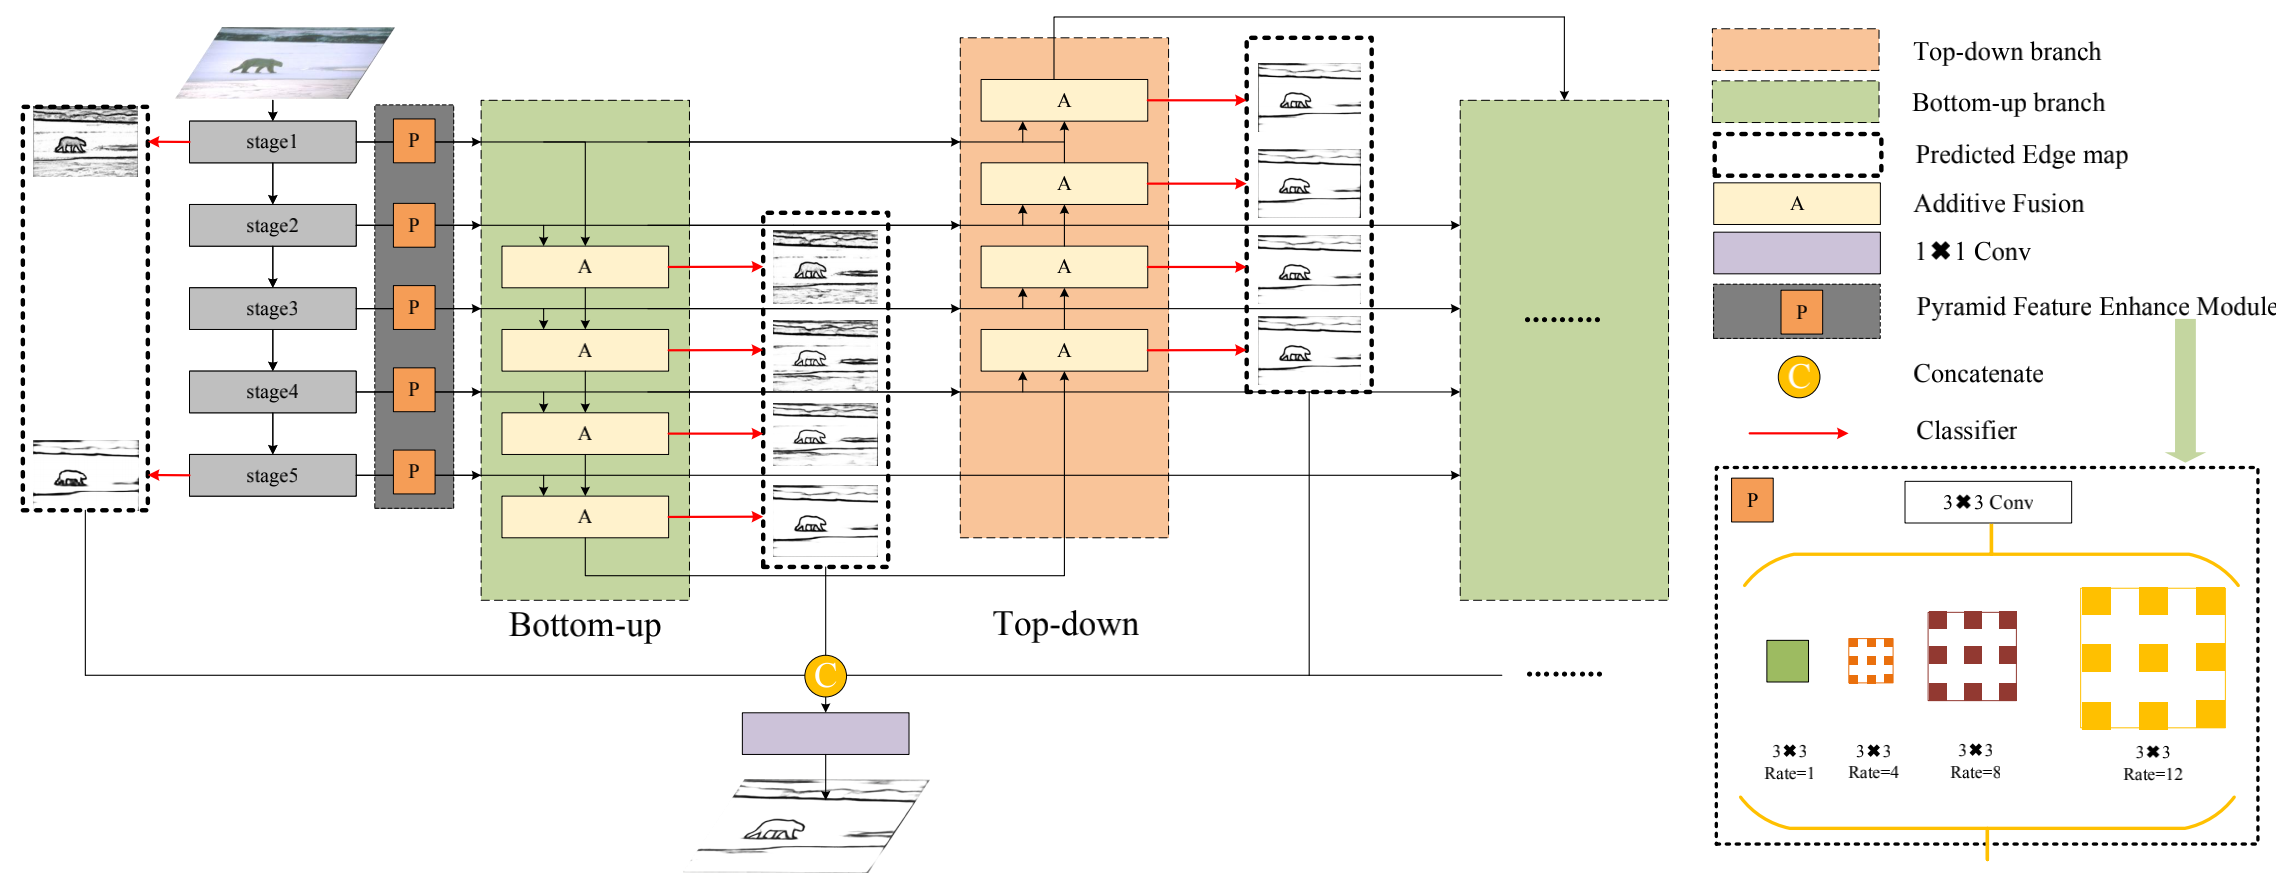
\includegraphics[width=1.0\textwidth]{graph/framework.pdf}
    \caption{本文提出的长时间单目标跟踪系统框架。}
	\label{fig:framework}
\end{figure*}
本文提出一种新的长时间跟踪框架,命名为MegTrack,总体框架如图~\ref{fig:framework}所示。
在每一帧中,局部跟踪器将局部搜索区域作为输入然后输出被跟踪对象的边界框。然后,验证器评估当前跟踪结果的正确性。
如果输出验证分数大于预定义的阈值,跟踪器将继续
下一帧进行局部跟踪。
如果分数小于阈值,我们使用faster R-CNN检测器\cite{fasterrcnn2015}来
在下一帧中检测所有可能的候选对象,并针对每个候选对象裁剪局部搜索区域。
然后,SiamPRN\cite{siamrpn++}模型将每个区域作为输入,输出对应的候选框。
这些包围框被发送给验证器,用于识别包围框内目标是否存在。
当验证器发现目标时,将重置局部跟踪器以适应当前目标的外观。
当验证器无法匹配到目标时,将启动one-shot检测器的全局搜索或者随机滑窗搜索。
在进入下一帧之前,所有的高置信度的目标历史信息被收集到一个目标容器中用于记录目标在跟踪过程中的外观形态大小的变化。
最后,容器中的样本将用于指导在线跟踪器和在线验证器的更新。

在这项工作中,我们实现了一个改进的AMT跟踪器,作为我们的局部跟踪器。该改进的跟踪模块应用了AMT算法中的分类分支用于定位目标
\footnote{在\ref{cap2}中提出的AMT跟踪器的尺寸估计分支是通过一个离线训练的实例个体级别IoU-Net实现的。}。在实际应用中,
我们发现SiamMask\cite{SiamMask}可以提供更加准确的尺度估计,可能是由于该方法是基于更强的像素级别标注训练得到的。
我们使用RTMDNet方法\cite{RTMDNet}作为我们的验证器,并对其进行验证
阈值设置为0。

与最近的排名靠前的长期目标跟踪器相比,我们的框架的主要力量在于嵌入一个全局one-shot实例检测器,一个在线更新的本地跟踪器
和一个在线验证器进入长时间目标跟踪框架中。这个想法让长时间目标跟踪解决方案受益于短期跟踪器最近的出色发展,
并尽可能将短期和长期跟踪问题统一起来。
一个不足之处在于,在线更新的风险会因为长期不确定的观测结果而放大(因为除了第一个帧之外的任何帧的结果都没有绝对可靠的跟踪精度)。
在后续的跟踪过程中,模型都处于一种无监督信息的状态。因此,我们提出了一种新的维护容器样本的方法来解决这个问题获得更稳健的跟踪性能。

\subsection{在线更新的验证模型}
在每一帧中,检测器或者跟踪器$\mathcal{R}$会回归局部搜索区域中的一系列候选框,它们的分数衡量候选框与对象模板之间的相似性。
然后,验证器$\mathcal{V}$在线学习分类边界,进一步判断最相似的候选框物体是真正的目标还是干扰物。
最后的置信分数是由$\mathcal{R}$和$\mathcal{V}$的分数的集成输出的,
它表示被跟踪的对象在当前帧中是\emph{present}还是\emph{absent}的概率分数。
如果需要,这个分数将被用来调用图像范围的重新检测方案。

\noindent
\textbf{容器样本收集策略:} 具有最高相似分数的候选框首先被裁剪出来并调整为$107\times107$,然后通过验证器网络$\mathcal{V}$进行验证。
该网络在线学习分类函数以进一步过滤跟踪过程中出现的干扰框,其中$c_i$表示第$i$个候选框。
如果将最相似的候选框分类为前景,则提出的跟踪器将获取候选框作为当前帧的跟踪结果$c^*$。
否则,$\mathcal{V}$从候选池中($[c_1, c_2, ... , c_{N_r}]$,$N_r$是需要考虑的候选框的个数)选择以比其他候选前景更高的相似度的前景候选对象作为跟踪结果。

\noindent
\textbf{验证器的网络模型构成:} 跟踪器或者one-shot检测器网络$\mathcal{R}$生成类似于对象模板的前景候选对象。
然而,生成的候选框可能包含导致目标对象模板发生质变的干扰因素。
直接针对特定对象更新$\mathcal{R}$是不合适的,
因为随着跟踪过程的进行,误差不可避免地会累积。
因此,一种合理的方式是保持$\mathcal{R}$固定,以保证可靠的相似性
度量并为候选对象引入额外的验证网络$\mathcal{V}$作为评估。
$ \mathcal{V}$的架构类似于RTMDNet~\cite{RTMDNet},以VGGM作为骨架网络。
它以一个$107 \times 107$ 的碎片区域作为输入和输出两个神经元指示
前景和背景的概率。
关于网络架构的更多细节可以在~\cite{RTMDNet}中找到。

与原始RTMDNet类似,我们更新了的最后三个卷积层
通过网络在线训练出一种基于softmax的强分类器,能够区分不同的
前景与背景的有效区别。
通过在线更新,$\mathcal{V}$帮助本文使用的局部跟踪器和one-shot检测器处理
跟踪过程中的各种杂乱干扰背景。
由于训练样本由跟踪器或one-shot检测器$\mathcal{R}$和验证器$\mathcal{V}$共同评估,
$\mathcal{V}$不太可能由于不适当的更新而崩溃。

\subsection{跟踪系统的逻辑和策略}
在推理阶段,局部跟踪器和one-shot检测器网络的参数是固定的。用于匹配的对象模板是在第一帧中给出的groundtruth。
我们仅以类似于原始RTMDNet的方式更新验证器网络\cite{RTMDNet}。

当需要重新定位目标时,本文提出的跟踪系统会启用全局搜索模式,启用GlobalTrack进行全局的one-shot检测搜索,
若有置信度高于阈值的候选框或候选区域,
将会启用验证器进行进一步验证。该跟踪器首先在搜索区域内搜索被跟踪对象,搜索区域面积为4倍的对象大小。
在每一帧中得到最佳候选对象后,我们就可以考虑被跟踪对象
为\emph{present}或\emph{absent},根据其置信度评分确定
如何在下一帧中搜索目标。如果置信度${S_c}$低于$0.3$的阈值,跟踪器认为目标在当前帧为\emph{absent}
,并在下一帧调用全局搜索模式。
否则,跟踪器将被跟踪的对象在当前帧中视为\emph{present}并继续下一帧采用局部跟踪器AMT进行跟踪。
全局和局部的跟踪搜索模式在长时间跟踪过程中会基于最佳候选框和候选区域的置信度评分动态切换,
这表明追踪器是否找到可靠的候选框对象。

在本文研究中,选取候选对象在每一帧中的置信度值${S_c}$
由跟踪器分数${S_r}$和验证器分数${S_v}$定义:
\begin{equation}
    {S_c} = \left\{ \begin{gathered}
    1.0,\;\;{S_v} > {\theta _{{v'}}}\;or\;{S_r} > {\theta _{{r'}}},{S_v} > 0 \hfill \\
    0,\;\;\;\;\;{S_r} < {\theta _r},{S_v} < 0 \hfill \\
    {S_r},\;\;\;otherwise \hfill \\ 
    \end{gathered}  \right., 
    \label{eq-confidence}
\end{equation}
其中$\theta_{v'} = 20.0$, $\theta_{r'} = 0.5$和$\theta_r = 0.3$。 
公式(\ref{eq-confidence})的原理包括:(1)当$\mathcal{V}$为
很有信心时($ {S_v} >{\theta _{{r'}}},{S_v} > 0$)或$\mathcal{R} $和$\mathcal{V}$
都有足够的信心(${S_r} > {\theta _{{r'}}},{S_v} > 0$),我们的跟踪器输出置信度指数为$1.0$;
(2)当$\mathcal{R}$和$\mathcal{V}$都给出负反馈时,跟踪器
返回$0$的置信度;
(3)否则,跟踪器的置信度将于跟踪器或者检测器的置信度一致($S_c = S_r$)。

当$\mathcal{R}$和$\mathcal{V}$都不能找到任何高度相似的候选区域
与分类置信度时,我们的跟踪器认为被跟踪的对象不在视野内,并在整个图像中搜索它。
除非跟踪器找到一个让$\mathcal{R}$和
$\mathcal{V}$都能得出高置信度的区域,跟踪器将当前帧中的目标视为\emph{absent}。
因为局部跟踪器和全局oneshot检测器$\mathcal{R}$是固定的(参数和目标模板)
在跟踪过程中,它不会累积误差,并能始终提供可靠的相似度评估。
$\mathcal{V}$将会动态地适应变化,以及收集的不准确的样本
在某种程度上,在线更新可以通过$\mathcal{R}$进行正则化。
通过使用了具有泛化性的$\mathcal{R}$和具有判别性的$\mathcal{V}$之间的互补
,该跟踪器能够有效地在长时间序列中进行单目标的跟踪。



\section{实验结果与分析}
我们的跟踪器是在PC机上使用Pytorch~\cite{pytorch}实现的
配备Inter i9 CPU (64G RAM)和NVIDIA GTX 2080 Ti。
平均追踪速度是22fps。
我们在VOT-2020数据集和OxUvA长期目标跟踪数据集~\cite{OxUvA}上对所提出的方法进行了评估~\cite{kristan2019seventh}
。详细的比较如下。

\subsection{在VOT2020数据集上的实验结果}
在视觉目标跟踪中提出了VOT-2020数据集~\cite{kristan2019seventh}
(VOT)挑战2018评估长期追踪器,包括$50$个挑战
各种物体的序列(如:人、汽车、摩托车、自行车和动物)
总帧长$215294$帧。每一种平均包含
10个长期目标消失,平均持续50帧。因此,该
数据集可以充分评估跟踪器的长期跟踪能力,这是必不可少的
在野外追踪。与VOT2018LT~\cite{VOT18}相比,VOT2020LT的引入带来了更多的挑战
15个更困难的视频和一些不常见的目标(如,船,公牛,和降落伞)。
遵循VOT2020~\cite{kristan2019seventh}的评估协议,跟踪精度
使用(\textbf{Pr})、recall (\textbf{Re})和\textbf{F-score}度量进行精度评估。
根据精度和召回度,定义阈值F-measure $F(\tau_{\theta})$为:
\begin{equation}
    \label{Fscore}
    F(\tau_{\theta}) = 2Pr(\tau_{\theta})Re(\tau_{\theta}) / (Pr(\tau_{\theta}) + Re(\tau_{\theta})), 
\end{equation}
其中$\tau_{\theta}$是官方使用的阈值。 然后,F-score被定义为F-measure图在所有阈值上的最高分数
$\tau_{\theta}$(即在跟踪器特定的最优阈值处取得的)。这种方式可以避免任意手动设置阈值,以鼓励公平评估。
在VOT2020中,\textbf{F-score}是主要的长期跟踪测量指标和用于排名不同的跟踪器。
此外,还采用了再检测实验的结果来进行比较
跟踪器,包括重新检测所需的平均帧数(\textbf{frames})
序列重新检测成功的百分比(\textbf{Success})。
详细的比较报告在Table~\ref{tab-vot20lt}中。结果表明,本文提出的跟踪器MegTrack比其他
所有比较的跟踪器的性能都要好得多。特别的,使用本文提出的MetaMixUp预训练方法模型作为主干特征提取网络,
我们获得了更加强大的跟踪器,MegTrack+,在F-Score指标上都取得了最优的结果,实验实例效果图见图\ref{fig:example}。
\begin{table}[htbp!]
    \caption{本文提出的长时间单目标跟踪器和state-of-the-art方法在VOT2020LT数据集上的性能比较。 
    最佳三种结果以\textcolor{red}{\textbf{red}},
    \textcolor{blue}{\textbf{blue}}和\textcolor{green}{\textbf{green}}三种颜色分别展示。
    所有的跟踪器根据\textbf{F-score}从上到下进行了排列。}
    \label{tab-vot20lt}
    \vspace{-3mm}
    \small
    \begin{center}
    \begin{tabular}{cccc}
    \hline
    \textbf{Tracker} & \textbf{F-score}                      & \textbf{Pr}                           & \textbf{Re}                           \\ \hline
    \textbf{MegTrack+(Ours)}             & {\color[HTML]{FE0000} \textbf{0.691}} & {\color[HTML]{3166FF} \textbf{0.701}} & {\color[HTML]{FE0000} \textbf{0.681}} \\
    \textbf{MegTrack(Ours)}             & {\color[HTML]{3166FF} \textbf{0.687}} & {\color[HTML]{FE0000} \textbf{0.703}} & {\color[HTML]{3166FF} \textbf{0.672}} \\
    SiamRPN++        & {\color[HTML]{32CB00} \textbf{0.629}} & {\color[HTML]{32CB00} \textbf{0.649}} & {\color[HTML]{32CB00} \textbf{0.609}} \\
    SPLT             &  0.616 & 0.633                                 & 0.600 \\
    MBMD              & 0.610                                 & 0.634                                 & 0.588                            \\
    DaSiam\_LT       & 0.607                                 & {\color[HTML]{000000} 0.627}          & 0.588       \\
    MMLT                & 0.546                                 & 0.574                                 & 0.521                            \\
    LTSINT              & 0.536                                 & 0.566                                 & 0.510                            \\
    SYT                   & 0.509                                 & 0.520                                 & 0.499                             \\
    PTAVplus           & 0.481                                 & 0.595                                 & 0.404                            \\
    FuCoLoT           & 0.480                                 & 0.539                                 & 0.432                             \\
    SiamVGG          & 0.459                                 & 0.552                                 & 0.393                             \\
    SLT                    & 0.456                                 & 0.502                                 & 0.417                             \\
    SiamFC              & 0.433                                 &  0.636 & 0.328  \\
    SiamFCDet        & 0.401                                 & 0.488                                 & 0.341                              \\
    HMMTxD         & 0.335                                 & 0.330                                 & 0.339                               \\
    SAPKLTF          & 0.323                                 & 0.348                                 & 0.300                               \\
    ASMS                & 0.306                                 & 0.373                                 & 0.259                               \\
    \hline
    \end{tabular}
    \end{center}
    \vspace{-5mm}
\end{table}


\begin{figure*}[htp!]
	\centering  
	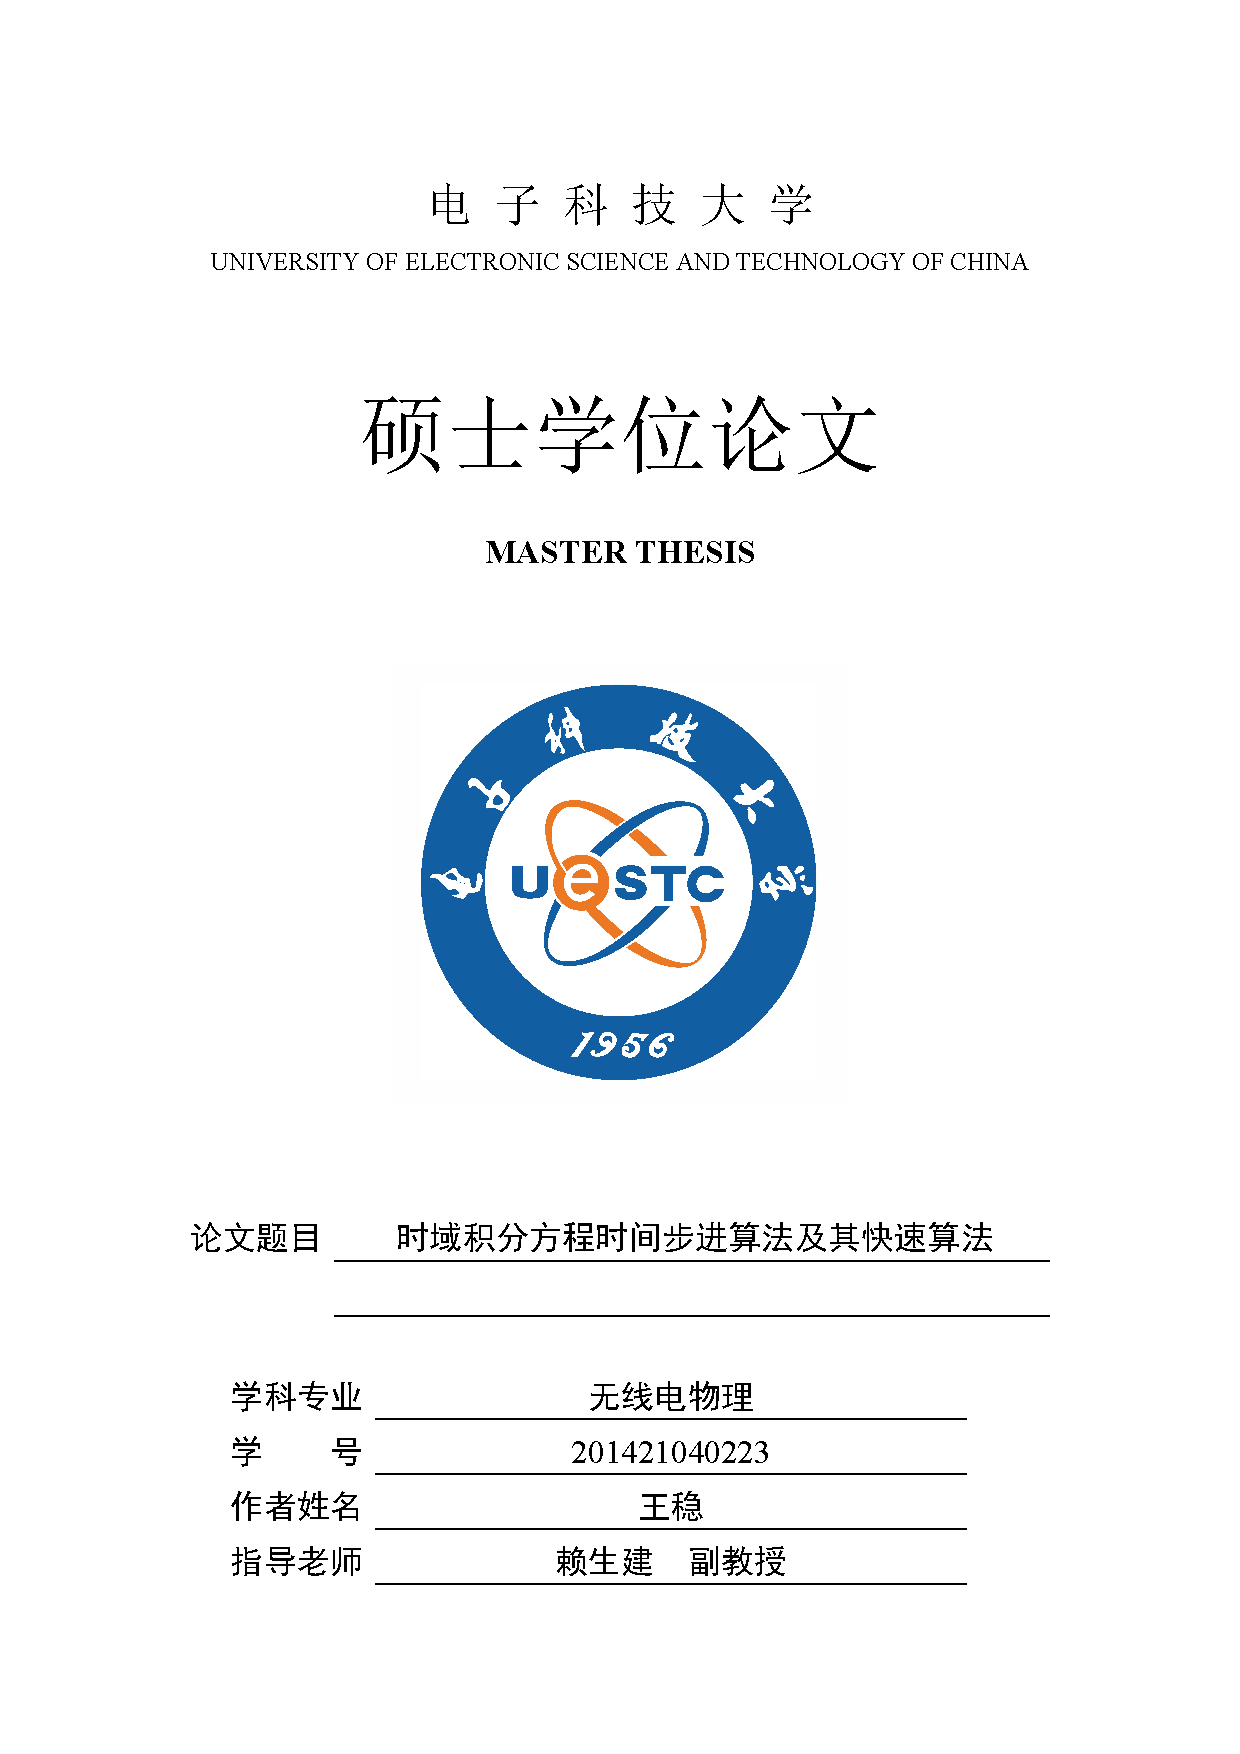
\includegraphics[width=1.0\textwidth]{graph/example.pdf}
    \caption{在VOT2020上的实验结果实例。}
	\label{fig:example}
\end{figure*}




\subsection{在OxUvA长时间跟踪数据集上的实验结果}
OxUvA长期数据集~\cite{OxUvA}由$337$段视频中的$366$种跟踪对象组成,视频从YoutubeBB数据集选择得到。
tracklet以$1$Hz的频率标记,这与YoutubeBB相同。
在这个数据集中,每个视频平均持续$2.4$分钟,比
OTB-100~\cite{OTB15}(最流行的短期跟踪数据集)长7倍。
除了短期跟踪的挑战性因素,严重的视线外丢失和完全遮挡
引入了额外挑战,这与从工业应用的需求是相近的。
将OxUvA数据集分成\emph{dev}和\emph{test}两个分别包含$200$和
$166$个跟踪轨道。利用这些子集,已经定义了两个挑战:
约束和开放。对于有约束的挑战,跟踪器只能使用
数据来自OxUvA \emph{dev}集合。
对于开放挑战,跟踪器可以使用任何公共数据集进行训练,除了YoutubeBB \emph{validation}集,因为OxUvA是由它构造的。
因为在OxUvA\cite{OxUvA}中报告的所有跟踪器都进行了公开测试
挑战,我们也进行了公开挑战的实验,公平比较。
遵循OxUvA~\cite{OxUvA}的评价基准,我们采用真
阳性率(\textbf{TPR}),真阴性率(\textbf{TNR}),最大
几何平均值(\textbf{MaxGM})来比较不同的跟踪器。
\textbf{TPR}度量\emph{present}对象被报告为\emph{present}的比例,而\textbf{TNR}度量\emph{absent}
对象被报告为\emph{absent}的比例。
\textbf{MaxGM}定义为:
\begin{equation}
    \label{MaxGM}
    \begin{array}{l}
    \mathbf{MaxGM} \\ 
    = \mathop {\max }\limits_{0 \le p \le 1} \sqrt {((1 - p) \cdot \mathbf{TPR})
    ((1 - p) \cdot \mathbf{TNR} + p)}\\ 
    \end{array}, 
\end{equation}
该评估方法提供了用于比较不同的跟踪器的更多信息和
用来对它们进行排序。较大的\textbf{MaxGM}值意味着更好的性能。实验的结果表格如\ref{tab:oxuva}所示。
我们可以看到我们的追踪器在\textbf{MaxGM}和\textbf{TPR}达到了排名第一的位置
同时在\textbf{TNR}上保持了具有竞争力的性能。
在同一网络框架下使用基于MetaMixUp数据增强方法训练的预训练模型
能进一步促进跟踪器的性能,MegTrack+在主要指标上均取得了最优的结果。
特别是,我们的跟踪器在所有比较跟踪器中有最好的性能
对于\textbf{MaxGM},它是OxUvA数据集上最重要的度量
。
与第二好的方法(SPLT)相比,我们的跟踪器获得了较好的跟踪性能,相比之下取得了,
显著改善,在\textbf{MaxGM}中相对增加$12.29\%$。

\begin{table}[h]
    \caption{本文提出的跟踪器与当前领先的跟踪器在OxUvA数据集上的性能评价。
    各个指标最佳的三个结果分别会被表示为\textcolor{red}{\textbf{red}}, \textcolor{blue}{\textbf{blue}}
    and \textcolor{green}{\textbf{green}}颜色。跟踪器会根据\textbf{MaxGM}的值从高到低进行排序。}
    \label{tab:oxuva}
    % \vspace{-3mm}
    \begin{center}
    \small
    \begin{tabular}{cccc}
    \hline
    \textbf{Tracker} & \textbf{MaxGM}                        & \textbf{TPR}                          & \textbf{TNR} \\
    \hline
    \textbf{MegTrack+}    &\textcolor{red}{\textbf{0.751}}  &\textcolor{red}{\textbf{0.749}} &\textcolor{green}{\textbf{0.754}} \\
    \textbf{MegTrack}    &\textcolor{blue}{\textbf{0.745}}  &\textcolor{blue}{\textbf{0.736}} &0.749 \\
    SPLT                &\textcolor{green}{\textbf{0.622}} &0.498          &\textcolor{blue}{\textbf{0.776}} \\
    GlobalTrack    &0.603                                    &0.574 & 0.633\\
    MBMD            &0.544                                  &\textcolor{green}{\textbf{0.609}} &0.485 \\
    %
    SiamFC+R      & 0.454                                 & 0.427                                 & 0.481                                 \\
    TLD                & 0.431                                 & 0.208                                & \textcolor{red}{\textbf{0.895}} \\
    LCT                & 0.396                                 & 0.292                                 & 0.537                                 \\
    MDNet            & 0.343                                 & 0.472                                & 0                                     \\
    SINT               & 0.326                                 & 0.426                                & 0                                     \\
    ECO-HC         & 0.314                                 & 0.395                                & 0                                     \\
    SiamFC           & 0.313                                 &0.391                                 & 0                                     \\
    EBT                & 0.283                                 & 0.321                                 & 0                                     \\
    BACF             & 0.281                                 & 0.316                                 & 0                                     \\
    Staple             & 0.261                                 & 0.273                                 & 0                                     \\
    \hline
    \end{tabular}
    \end{center}
\end{table}

\subsection{消融实验}
在这个小节中,我们进行消融分析来评估我们跟踪器中不同的组成部分。
在不同的实验设置下,我们设计了四种不同的跟踪器,分别命名为“w/o verifier”,“w/o results pool”,
“w/o one-shot det”和“w/o siamrpn”。
这些概念的含义解释如下:(1) “w/o verifier”表示不包含验证器,只使用localtracker和one-shot检测器的结果
作为局部跟踪和全局检测的置信度指标;(2)“w/o results pool”
表示验证器不采用results pool的采样策略进行验证器的在线更新,而只使用最后一次的结果进行数据增强后更新验证器;
(3) “w/o one-shot det”表示不使用one-shot检测器进行全局目标检测,但丢失目标后采用全局滑窗的方法进行重新检测;
(4)“w/o siamrpn”表示不使用siamrpn网络进行重检测的结果集成,直接采用one-shot检测器的结果,而不进行框的修正。
\begin{table}[!h]
    \caption{在VOT-2020数据集上进行消融分析。 
    最好的结果会被标记为\textcolor{red}{\textbf{red}}颜色。 }
    \vspace{-1mm}
    \begin{center}
    \begin{tabular}{p{3.8cm}<{\centering}p{1.2cm}<{\centering}
    p{0.7cm}<{\centering}p{0.7cm}}
    \hline
    \textbf{Tracker} & \textbf{F-score} & \textbf{Pr} & \textbf{Re} \\
    \hline
    Ours  & \textbf{\textcolor[rgb]{1,0,0}{0.687}} 
    & \textbf{\textcolor[rgb]{1,0,0}{0.703}} & \textbf{\textcolor[rgb]{1,0,0}{0.672}}\\
    %\hline
    Ours w/o verifier & 0.613 & 0.581 & 0.637\\
    %\hline
    Ours w/o results pool & 0.642 & 0.682 & 0.601\\
    %\hline
    Ours w/o one-shot det & 0.582 & 0.630 & 0.540\\
    Ours w/o siamrpn & 0.651 & 0.643 & 0.666\\
    \hline
    \end{tabular}
    \end{center}
    \label{tab:ablation}
    \vspace{-3mm}
\end{table}

在VOT-2020上进行实验的不同结构的结果见表\ref{tab:ablation}所示。从表中我们可以发现以下结论。
(1)“Ours w/o verifier”和“Ours”比较下,我们可以产生结论,我们提出的验证器方案能够大幅度的提升模型的性能,
尤其在准确率方面,在验证器的加持下提高了跟踪结果的精度。
(2)比较“Ours w/o results pool”和“Ours”发现,本文提出的记录结果的容器策略能够大幅度的提高模型对目标在跟踪过程中
变化的适应性,从而提高了模型的召回率。
(3)“Ours”和“Ours w/o one-shot det”之间的性能比较充分的说明了本文提出的one-shot检测器方案的重要性,
在没有one-shot检测器的条件下,跟踪器模型的召回率大幅下降,重新检测的能力大幅下降。
(4)使用siamrpn模型对one-shot检测器的结果进行进一步的修正,能够提高跟踪结果的精度,使得局部跟踪器和验证器
都能输入更精准的候选框进行进一步的判定,从而提升整体框架的性能。

\section{本章小结}
本章工作提出了一个新的长期目标跟踪框架,框架包含了局部跟踪器,one-shot检测器作为全局搜索器以及可在线更新的验证器。
one-shot全局搜索器通过离线训练得到,在线跟踪阶段是固定的,可以有效的候选框建议和可靠的相似度估计
的同时不会在长序列中累积错误跟踪偏差。此外,利用验证网络模块对
生成的候选对象进行评估并在跟踪过程种进行网络参数微调以捕获
外观变化。局部搜索和全图像搜索之间的动态切换方案和
重新检测的设计使得跟踪系统能基于一个由回归和验证网络统一化的输出确定预测置信值。




\chapter{全文总结与展望}

\section{全文总结}
本文以视觉单目标跟踪方法为研究背景,主要短时局部单目标跟踪算法和长时间单目标跟踪算法进行了深入研究。
由于视觉目标跟踪对模型特征提取判别性的高质量需求,本文提出一种基于元学习的Bilevel优化算法,
应用于图像增强MixUp的策略搜索,根据数据的先验分布,减少因为数据增强而导致的欠拟合现象,同时提高预训练模型的特征判别性质量
和抗干扰能力。由于预训练模型将用于有所跟踪器的骨架网络初始化和候选目标特征的提取,
因此预训练模型性能的提高将促进跟踪器的性能。

针对常用的短时目标跟踪问题,本文在第三章中给出了相关任务的数学模型,指出了该任务的主要问题是在对外观和运动模型施加的约束简化的,包括高斯窗口的限制下,
得到局部搜索区域中的最大响应位置,并通过回归模型进行目标尺寸大小的预测,同时给出了短时视觉单目标跟踪的定义。
然后介绍了与本文算法相关的局部跟踪器算法框架,发现了相关算法对目标的定位不准确,忽视了模型特征由于目标形变,旋转和干扰物影响引发的特征质量下降问题,
由于缺乏关键特征信息,无法提供准确的目标状态估计。因此本文提出了一种特征调制算法,从全局特征和局部关键特征进行融合,
我们将高级全局模板信息与低级局部建议信息进行编码,对目标本身和邻近环境都进行建模,
丰富了用于前后景分类和目标状态估计的特征信息。然后对文本提出的短时局部跟踪器的算法AMT进行了介绍,提出了一种基于Attention特征的相关滤波分类器的初始化方法,
可用于提供目标的粗定位并且减少了计算的时间复杂度提高跟踪响应速度。接着介绍了全局-局部特征调制模块,用于匹配模板和候选区域的特征相关性,调制模块对特征空间进行了有效的注意力权重分配,
得到全局目标特征,通过与局部候选特征的融合调制获得包含目标关键信息编码的特征图。同时本文在该章节还提出了一种结构化三元组损失函数,
从亮度,对比相似度和结构相似度全方位度量图像候选目标与模板目标之间的相似性。最后介绍了该局部跟踪器的离线训练方法和相关实验配置,以及在跟踪过程中的跟踪使用策略。
在消融实验和讨论部分,我们还介绍了本文特征调制的其他组合结构,并进行了分析讨论;另外通过对比实验展示了
本文的结构化三元组损失函数的有效性。最后还分别探索了在减少搜索空间约束和低帧率高速运动状态下,本文局部跟踪器的效果,
实验表明,与当前性能最好的跟踪器相比,本文局部跟踪器在这些极端条件下,仍能表现出稳定良好的性能。

在第四章中,介绍了本文设计的适用于长时间跟踪场景的单目标跟踪系统框架,本文首先介绍了one-shot检测器的概念和相关算法,
在one-shot检测器的加持下,提出了在长时间跟踪系统中加入one-shot检测器作为全局搜索的解决办法。
长期跟踪器的一个关键功能是在整个图像中搜索目标,以处理可能的目标缺失或跟踪失败。同时引入了一个可在线学习更新的验证器网络模块,
适应目标在跟踪过程中外观变化。最终提出了一套全局-局部跟踪一体化的长时间单目标跟踪系统框架。
本文将设计的框架分为局部跟踪和全局搜索两个部分。局部跟踪又局部跟踪器和验证器组成,
当发现存在目标时使用AMT进行局部跟踪。全局搜索器由one-shot检测器,另一个集成的局部跟踪器和验证器组成。
验证器在两个部分中都起着把关的作用,对候选结果进行筛选判断目标是否为所需跟踪的目标。
同时介绍了验证器的网络构成和跟踪过程中在线更新的策略。最后对本文提出的跟踪系统在两个权威的长时间跟踪数据集上进行实验,
均得到了当前业内最佳的效果,展示了本文算法的性能,还对算法的实验结果进行了可视化展示分析。

本文针对视觉单目标跟踪任务提出了一种改进预训练优化策略,一种改进的局部跟踪器特征调制模块和相关改进算法和
一种针对长时间单目标跟踪的系统框架。明确了算法模型的各模块和功能,对各个模块都进行了深入的实验研究和数学理论分析,
最后进行了实验的验证。本文针对视觉单目标跟踪提出的算法模型和相关优化算法对其他研究者甚至其他计算机科学领域的
科学研究或工程实践都具有参考价值。




\section{后续工作展望}
视觉单目标跟踪方法的研究近几年发展迅速,在本文研究工作的基础上,仍有以下方向值得进一步研究:
跟踪器的性能可以通过包括时间信息和空间信息来改善。
目前,跟踪界对RNN的研究还不多,所以使用类似RNN的架构能在多大程度上提高性能还不清楚。
由于缺乏训练数据的可用性,基于学习的跟踪算法很吃紧。
近年来,zero-shot学习和one-shot学习的研究主要是缓解数据限制问题,也是跟踪领域有待探索的新方向。
在检测跟踪框架中,由于有限的阳性样本,在线更新当前帧会导致过拟合问题。
对于长期跟踪,需要捕获所有目标形状变化的正目标斑块来学习完整的目标外观。生成对抗网络(GAN)有能力产生真实的图像。
在跟踪框架中加入GAN和强化学习也可以有效地提高跟踪性能,是一个很有前途的未来方向。
简而言之,跟踪器能够实时学习目标的形状、外观和几何形状,以及时间变化,这对实时跟踪至关重要。
因此,有必要在不损失精度的前提下获得较高的跟踪速度,这也是未来的一个发展趋势。

\thesisacknowledgement
在攻读硕士学位期间,首先衷心感谢我的指导老师申恒涛教授,在我的研究生生涯中给我提供很多指导与帮助,
为您的才学所折服,更为您磊落的人品所敬仰,“不负韶华”永记于心。

感谢沈复民教授,感谢您在我迷茫时的悉心开导为,我提供思路和宝贵意见和不计回报的辛勤培育。

感谢身在国外合作的胡国圣老师和陈德熊同学,一起工作不仅在学术上受益匪浅,在为人处事方面,
你们也一直给我分享经验,让我成长,变得更加成熟。

感谢实验室的小伙伴们,和团队的小伙伴相处公事留下了许多美好的点滴。

感谢家人,一路以来对我的生活上,学业上的支持,给与了我一个温暖、热情美好的成长环境,树立了我正确的人生观、价值观、世界观。
是我信心动力的来源,永远的后盾。

感谢在一起合作公事过的校外同学,为你们的才学所折服,受你们的谦和博学精神所影响。

感谢为本文提出意见的评审专家、老师和同学。

最后,再次感谢所有述及和未述及的人。

朝来庭下,光阴如箭。
别离难,不似相逢好。

\thesisappendix

% \chapter{中心极限定理的证明}

% \section{高斯分布和伯努利实验}


% Uncomment to list all the entries of the database.
% \nocite{*}

\thesisbibliography[large]{reference}

%
% Uncomment following codes to load bibliography database with native
% \bibliography command.
%
% \nocite{*}
% \bibliographystyle{thesis-uestc}
% \bibliography{reference}
%

\thesisaccomplish{publications}

% \thesistranslationoriginal
% \section{The OFDM Model of Multiple Carrier Waves}

% \thesistranslationchinese
% \section{基于多载波索引键控的正交频分多路复用系统模型}

\end{document}
